%
% exemplo genérico de uso da classe iiufrgs.cls
% $Id: iiufrgs.tex,v 1.1.1.1 2005/01/18 23:54:42 avila Exp $
%
% This is an example file and is hereby explicitly put in the
% public domain.
%
\documentclass[ppgc,tese,english,formais,babel]{iiufrgs}
% Para usar o modelo, deve-se informar o programa e o tipo de documento.
% Programas :
%   * cic       -- Graduação em Ciência da Computação
%   * ecp       -- Graduação em Ciência da Computação
%   * ppgc      -- Programa de Pós Graduação em Computação
%   * pgmigro   -- Programa de Pós Graduação em Microeletrônica
%
% Tipos de Documento:
%   * tc                -- Trabalhos de Conclusão (apenas cic e ecp)
%   * diss ou mestrado  -- Dissertações de Mestrado (ppgc e pgmicro)
%   * tese ou doutorado -- Teses de Doutorado (ppgc e pgmicro)
%   * ti                -- Trabalho Individual (ppgc e pgmicro)
%
% Outras Opções:
%   * english    -- para textos em inglês
%   * openright  -- Força início de capítulos em páginas ímpares (padrão da
%                   biblioteca)
%   * oneside    -- Desliga frente-e-verso
%   * nominatalocal -- Lê os dados da nominata do arquivo nominatalocal.def

% Use unicode
\usepackage[utf8]{inputenc}   % pacote para acentuação

% Necessário para que as tabelas tenham separador correto:
% '--' (travessão) ao invés de ':' (dois-pontos).
\usepackage{float}

% Necessário para incluir figuras
\usepackage{graphicx}           % pacote para importar figuras

\usepackage{times}              % pacote para usar fonte Adobe Times
% \usepackage{palatino}
% \usepackage{mathptmx}          % p/ usar fonte Adobe Times nas fórmulas

\usepackage[alf,abnt-emphasize=bf]{abntex2cite}	% pacote para usar citações abnt

% Packages added by Henrique Becker
\usepackage{multirow}
\usepackage{hyperref}
\usepackage{color}
\usepackage[table]{xcolor}
\definecolor{gray-table-row}{gray}{0.90}
\definecolor{gray-inner-row}{gray}{0.95}
% Packages for computer code
\usepackage{algorithm}
\usepackage{algpseudocode}
% Package for multiline comments
\usepackage{verbatim}
% For keeping tables in a single page (only for writing, not final doc)
\usepackage{adjustbox}
% Packages for formatting the mathematical formulation
\usepackage{mathtools}
\usepackage{amsmath}
\usepackage{amssymb}
\usepackage{bm} % for correct font and emphasis in formulation max/min
% For better treatment of nested lists.
\usepackage{enumitem}
% For better referencing (\cref, \Cref).
\usepackage[nameinlink]{cleveref}
\usepackage{longtable}

\usepackage{tikz}
\usetikzlibrary{patterns}
% The booktabs import below allow us to use cmidrule, which should replace
% cline in tables and avoid the extracolsep hack (which breaks rowcolors).
\usepackage{booktabs}
% We want to use \cref and \Cref correctly (i.e., cref in the middle of
% a sentence, and Cref only in the beginning of a sentence), but we also
% need to follow the standard that says that all references are capitalized
% independent of where they are in a sentence.
\crefname{chapter}{Chapter}{Chapters}
\crefname{section}{Section}{Sections}
% Fix the mess that is the theorem/definition environment defined by
% iiufrgs.cls (formais.def).
\crefname{envtheorem}{Theorem}{Theorems}
\crefname{envdefinition}{Definition}{Definitions}

\newif\iffinalversion
%\finalversiontrue
\newcommand{\newtext}[1]{\iffinalversion%
#1%
\else%
\textcolor{blue}{#1}%
\fi%
}
\newcommand{\oldtext}[1]{\iffinalversion%
\else%
\textcolor{red}{#1}%
\fi%
}
%\finalversiontrue

\newcommand{\isep}{\mathrel{{.}\,{.}}\nobreak} % for integer ranges
\newcommand{\bestcolumnemph}[1]{\textbf{#1}}

\usepackage{xhfill}% http://ctan.org/pkg/xhfill
%\newcommand{\ditto}{\multicolumn{1}{c}{\textquotedbl}}
\newcommand{\ditto}{\textquotedbl}

% Necessary for formulation layout workaround.
\newcommand{\pushright}[0]{\hskip \textwidth minus \textwidth}
\makeatletter
\newcommand{\specialcell}[1]{\ifmeasuring@#1\else\omit$\displaystyle#1$\ignorespaces\fi}

% Avoids problem with citet in section names (the name of the reference
% becomes all-caps and then it is not found in the bib file).
\def\citethopperthesis{\citet{hopper_thesis}}

%
% Informações gerais
%
\title{An enhanced formulation for guillotine 2D cutting problems
%\thanks{This study was financed in part by the Coordenação de Aperfeiçoamento de Pessoal de Nível Superior - Brasil (CAPES) - Finance Code 001}
}

\author{Becker}{Henrique}

% orientador e co-orientador são opcionais (não diga isso pra eles :))
\advisor[Prof.~Dr.]{Buriol}{Luciana Salete}
\coadvisor[Prof.~Dr.]{Araujo}{Olinto}

% a data deve ser a da defesa; se nao especificada, são gerados
% mes e ano correntes
%\date{maio}{2001}

% o local de realização do trabalho pode ser especificado (ex. para TCs)
% com o comando \location:
%\location{Itaquaquecetuba}{SP}

% itens individuais da nominata podem ser redefinidos com os comandos
% abaixo:
% \renewcommand{\nominataReit}{Prof\textsuperscript{a}.~Wrana Maria Panizzi}
% \renewcommand{\nominataReitname}{Reitora}
% \renewcommand{\nominataPRE}{Prof.~Jos{\'e} Carlos Ferraz Hennemann}
% \renewcommand{\nominataPREname}{Pr{\'o}-Reitor de Ensino}
% \renewcommand{\nominataPRAPG}{Prof\textsuperscript{a}.~Joc{\'e}lia Grazia}
% \renewcommand{\nominataPRAPGname}{Pr{\'o}-Reitora Adjunta de P{\'o}s-Gradua{\c{c}}{\~a}o}
% \renewcommand{\nominataDir}{Prof.~Philippe Olivier Alexandre Navaux}
% \renewcommand{\nominataDirname}{Diretor do Instituto de Inform{\'a}tica}
% \renewcommand{\nominataCoord}{Prof.~Carlos Alberto Heuser}
% \renewcommand{\nominataCoordname}{Coordenador do PPGC}
% \renewcommand{\nominataBibchefe}{Beatriz Regina Bastos Haro}
% \renewcommand{\nominataBibchefename}{Bibliotec{\'a}ria-chefe do Instituto de Inform{\'a}tica}
% \renewcommand{\nominataChefeINA}{Prof.~Jos{\'e} Valdeni de Lima}
% \renewcommand{\nominataChefeINAname}{Chefe do \deptINA}
% \renewcommand{\nominataChefeINT}{Prof.~Leila Ribeiro}
% \renewcommand{\nominataChefeINTname}{Chefe do \deptINT}

% A seguir são apresentados comandos específicos para alguns
% tipos de documentos.

% Relatório de Pesquisa [rp]:
% \rp{123}             % numero do rp
% \financ{CNPq, CAPES} % orgaos financiadores

% Trabalho Individual [ti]:
% \ti{123}     % numero do TI
% \ti[II]{456} % no caso de ser o segundo TI

% Monografias de Especialização [espec]:
% \espec{Redes e Sistemas Distribuídos}      % nome do curso
% \coord[Profa.~Dra.]{Weber}{Taisy da Silva} % coordenador do curso
% \dept{INA}                                 % departamento relacionado

%
% palavras-chave
%
\keyword{Combinatorial optimization}
\keyword{2D knapsack}
\keyword{Guillotine cuts}
\keyword{Mathematical formulation}

%
% inicio do documento
%
\begin{document}

\chapter{Hybridization with the restricted formulation}

This chapter proposes another symmetry-breaking change compatible with the formulations considered in~PREVIOUS CHAPTER. %\cref{XXX}.
This change further complicates the formulation, and the empirical results did not reveal an improvement as large as the previously discussed enhancements.
Therefore, the author chose to keep this change self-contained in this chapter.
The author is unaware of any previous application of the proposed change to unrestricted 2D guillotine problems.
The Cut-Position enhancement from~\cite{furini:2016} draws inspiration from the same broad idea: to get closer to a formulation for the (simpler) restricted problem while keeping optimality for the unrestricted problem.
However, the proposed change and the Cut-Position both approach this goal in distinct and complementary ways.

\section{The restricted problem and piece-outlining cuts}

A guillotine cutting problem is said to be \emph{restricted} if (i) each horizontal (vertical) guillotine cut must match the length (width) of a piece that fits into the plate, i.e., it happens at a \emph{restricted cut position}, and (ii) a piece of that length (width) is guaranteed to be obtained from the first child plate.
The concept of a \emph{restricted} variant appears first in the context of the three-staged guillotine cutting problem.
The two-staged problem is inherently restricted: a cut that does not match the outline of a piece, or a cut that does not guarantee a piece extraction because it is not paired with a cut from the only other stage, is a cut that will not help to obtain any pieces before the two stages are over.
Only when the number of stages is three or more that an optimal solution to the unrestricted problem may require cuts without such clearly immediate purposes.
Our definition (at the start of the paragraph) can be seen as an extension of the concept for the problem with unlimited stages.
Applying the concept of \emph{restricted} to unlimited stages is not new, \cite{furini:2016} already does it. \cite{furini:2016} also presents an intermediary variant which respects (i) but not (ii), this variant can be referred to as \emph{position-only} restricted problem.
The \emph{position-only restricted problem} is the one solved by the \emph{restricted priced} in~PREVIOUS CHAPTER%\cref{xxx}.

%The (position-only) restricted problem may be required (or prefered) because of precision problems dependent on available cutting technology~\citep{furini:2016}, however it is also used an as high-cost high-quality heuristic for the unrestricted problem.
The restricted problem has at least two performance advantages over the unrestricted problem.
The first advantage is related to the number of restricted cut positions: the number of cuts positions in any plate is bounded by the number of pieces (i.e., linear on the input), and not pseudo-polynomial (i.e., bounded by plate dimensions), even if the number of plates themselves is still pseudo-polynomial.
The second advantage is related to the piece extraction requirement.
There is no optimality loss if, after a cut at a restricted position, it is immediately determined that, if necessary, the first child plate will be cut again in the next stage to obtain the associated piece.
The possibility of joining two decision variables together has led previous prior on the restricted problem, as \cite{silva:2010}, to redefine \emph{cut} to mean \emph{one or two guillotine cuts associated a priori to a piece type and which outline and obtain a piece-sized plate that cannot be further cut}.
The guillotine cuts considered up until now may incidentally outline and obtain a piece-sized plate as their child plates.
However, they are not a priori associated with a single piece type, nor do they guarantee their first child plate (if piece-sized) cannot be further cut.
In this chapter, the text distinguishes between these two kinds of cuts to avoid confusion.
The single and unassociated cuts considered up until now will be referred to as \emph{basic guillotine cuts} (or BGCs for short), and this new definition of cut will be referred to as \emph{piece-outlining cuts} (or POCs for short).
\Cref{fig:piece_outlining_cut} may help the visualization of the \emph{piece-outlining cuts}.

\begin{figure}[h]
  \caption{Piece-outlining cuts}
  \center
  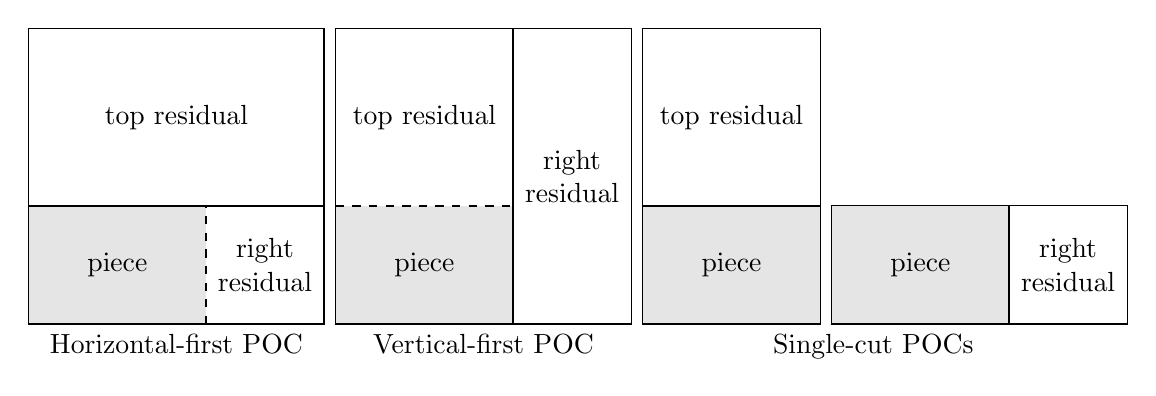
\begin{tikzpicture}[scale=0.15]
\def\piececolor{gray!20}
\def\labelxshift{12.5}
\def\labelyshift{0}
\def\labelfontsize{\normalsize}
\begin{scope}[shift={(0, 0)}] % FIRST ROW
\begin{scope}[shift={(0, 0)}] % FIRST IMAGE

\fill[\piececolor] (0, 0) rectangle +(15, 10);
\draw[thick, black] (0, 10) -- (25, 10);
\draw[dashed, thick, black] (15, 0) -- (15, 10);
\draw (0,0) rectangle +(25, 25);

\node [align=center, font=\labelfontsize\selectfont] at (7.5, 5) {\labelfontsize piece}; %{\labelfontsize piece-sized \\ \labelfontsize plate};
\node [align=center, font=\labelfontsize\selectfont] at (12.5, 17.5) {\labelfontsize top residual};
\node [align=center, font=\labelfontsize\selectfont] at (20, 5) {right\\residual};

\node [below] at (\labelxshift, \labelyshift) {\labelfontsize Horizontal-first POC};
\end{scope}

\begin{scope}[shift={(26, 0)}] % SECOND IMAGE

\fill[\piececolor] (0, 0) rectangle +(15, 10);
\draw[dashed, thick, black] (0, 10) -- (15, 10);
\draw[thick, black] (15, 0) -- (15, 25);
\draw (0,0) rectangle +(25, 25);

\node [align=center, font=\labelfontsize\selectfont] at (7.5, 5) {\labelfontsize piece}; %{\labelfontsize piece-sized \\ \labelfontsize plate};
\node [align=center, font=\labelfontsize\selectfont] at (7.5, 17.5) {\labelfontsize top residual};
\node [align=center, font=\labelfontsize\selectfont] at (20, 12.5) {right\\residual};

\node [below] at (\labelxshift, \labelyshift) {\labelfontsize Vertical-first POC};
\end{scope}

\begin{scope}[shift={(52, 0)}] % THIRD IMAGE

\fill[\piececolor] (0, 0) rectangle +(15, 10);
\draw[thick, black] (0, 10) -- (15, 10);
%\draw[dashed, thick, black] (15, 0) -- (15, 10);
\draw (0,0) rectangle +(15, 25);

\node [align=center, font=\labelfontsize\selectfont] at (7.5, 5) {\labelfontsize piece}; %{\labelfontsize piece-sized \\ \labelfontsize plate};
\node [align=center, font=\labelfontsize\selectfont] at (7.5, 17.5) {\labelfontsize top residual};
\end{scope}

\begin{scope}[shift={(68, 0)}] % FOURTH IMAGE

\fill[\piececolor] (0, 0) rectangle +(15, 10);
%\draw[dashed, thick, black] (0, 10) -- (15, 10);
\draw[thick, black] (15, 0) -- (15, 10);
\draw (0,0) rectangle +(25, 10);

\node [align=center, font=\labelfontsize\selectfont] at (7.5, 5) {\labelfontsize piece}; %{\labelfontsize piece-sized \\ \labelfontsize plate};
\node [align=center, font=\labelfontsize\selectfont] at (20, 5) {right\\residual};
\end{scope}
\node [below, align=center, font=\labelfontsize\selectfont] at (71.5, 0) {\labelfontsize Single-cut POCs};

\end{scope}
\end{tikzpicture}

  \legend{Souce: the author.}
  \label{fig:piece_outlining_cut}
\end{figure}

While a POC constituted by two BGCs may be considered as a single decision by a solving method and may be seen as happening in succession, in practice, stage restrictions may change the order a cutting machine perform them.
However, these real-world details do not impact our modelling and will not be discussed in this chapter.
Essentially, each piece type that fits into a plate has two POCs associated with it.
One POC that does the horizontal guillotine cut first and then obtains the piece from the first child plate through a vertical cut (if necessary).
This POC always leaves a \emph{top residual plate} (second child plate of the first cut) and often a \emph{right residual plate} (second child plate of the second cut).
The other POC is the same except that the vertical cut is done first (i.e., always leaving a right residual and often a top residual plate).
Finally, the piece-sized plate obtained by a POC is the first child plate of the second cut, if the second cut exists, otherwise just the first child plate of the only cut.
The piece-sized plate is either immediately regarded as an obtained piece (already enforcing a rule of the restricted problem), or it may be considered waste (e.g., the cutting stock problem often allow piece overproduction).
However, the piece-sized plate is \emph{never} treated as an intermediary plate that could be further cut.

A caveat of the coupled representation mentioned above is that, for some instances of the restricted problem, the number of POCs may be larger than the number of restricted cut positions.
In general, each piece type that fits into a plate has two POCs\footnote{The exception happens when the piece type shares the length or the width with the plate and, consequently, both POCs are equivalent and can be considered the same.} (vertical-first and horizontal-first).
A horizontal (vertical) BGC at a restricted position is shared by all piece types with the same length (width).
However, the main advantage of the coupled representation comes from breaking symmetries not reducing the number of variables.
%For example, if a stripe of width~\(10\) is obtained by a BGC in the restricted problem, it may be used to obtain a single piece of width~\(10\) and four pieces of width~\(8\), and every permutation in the order of the pieces are obtained from the strip is a symmetry, the POC enforce the width~\(10\) piece is the first to be obtained, and that no other mechanism is necessary to guarantee that the piece will be obtained from such plate.

The POCs are a natural choice for the \emph{restricted} problem but not for the \emph{unrestricted} problem for mostly two main reasons.
The first reason is that, in the restricted problem, each horizontal (vertical) cutting position shares length (width) with at least one piece.
However, in the unrestricted problem, some cutting positions can only be reached by combining many pieces.
The second reason is that the definition of the \emph{restricted} problem guarantees that employing only POCs cannot lead to optimality loss; the same is not true for the unrestricted problem (see \cref{fig:distinctions_restricted_unrestricted}).

\begin{figure}[h]
  \caption{Distinctions between, restricted, position-only restricted, and unrestricted problems.}
  \center
  \usetikzlibrary{patterns}
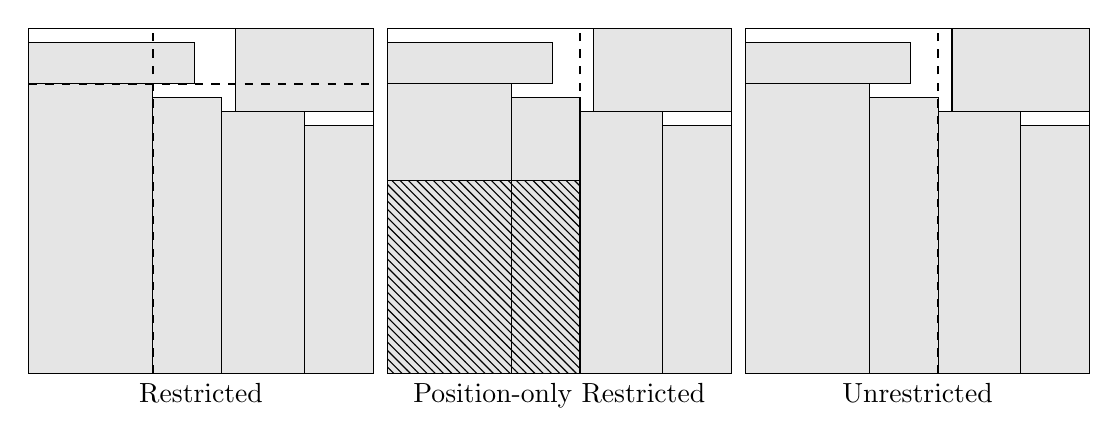
\begin{tikzpicture}[scale=0.175]
\def\piececolor{gray!20}
\def\labelxshift{12.5}
\def\labelyshift{0}
\def\labelfontsize{\normalsize}

\begin{scope}[shift={(0, 0)}] % FIRST ROW
\begin{scope}[shift={(0, 0)}] % FIRST IMAGE
\draw (0,0) rectangle +(25, 25);

%\draw[fill=\piececolor] (0,0) rectangle +(6, 19);
%\draw[fill=\piececolor] (6,0) rectangle +(5, 18);
\draw[fill=\piececolor] (14,0) rectangle +(6, 19);
\draw[fill=\piececolor] (20,0) rectangle +(5, 18);
\draw[fill=\piececolor] (0,0) rectangle +(9, 21);
\draw[fill=\piececolor] (9,0) rectangle +(5, 20);
%\draw[fill=\piececolor] (0,19) rectangle +(10, 6);
\draw[fill=\piececolor] (15,19) rectangle +(10, 6);
\draw[fill=\piececolor] (0,21) rectangle +(12, 3);

\draw[dashed, thick, black] (0, 21) -- (25, 21);
\draw[dashed, thick, black] (9, 0) -- (9, 25);


\node [below] at (\labelxshift, \labelyshift) {\labelfontsize Restricted};


\draw (0,0) rectangle +(25, 25);
\end{scope}

\begin{scope}[shift={(26, 0)}] % SECOND IMAGE
\draw (0,0) rectangle +(25, 25);

%\draw[fill=\piececolor] (0,0) rectangle +(6, 19);
%\draw[fill=\piececolor] (6,0) rectangle +(5, 18);
\draw[fill=\piececolor] (14,0) rectangle +(6, 19);
\draw[fill=\piececolor] (20,0) rectangle +(5, 18);
\draw[fill=\piececolor] (0,0) rectangle +(9, 21);
\draw[fill=\piececolor] (9,0) rectangle +(5, 20);
%\draw[fill=\piececolor] (0,19) rectangle +(10, 6);
\draw[fill=\piececolor] (15,19) rectangle +(10, 6);
\draw[fill=\piececolor] (0,21) rectangle +(12, 3);

\draw[pattern=north west lines] (0,0) rectangle +(14, 14);
\draw[dashed, thick, black] (14, 0) -- (14, 25);

\node [below] at (\labelxshift, \labelyshift) {\labelfontsize Position-only Restricted};
\end{scope}

\begin{scope}[shift={(52, 0)}] % THIRD IMAGE
\draw (0,0) rectangle +(25, 25);

%\draw[fill=\piececolor] (0,0) rectangle +(6, 19);
%\draw[fill=\piececolor] (6,0) rectangle +(5, 18);
\draw[fill=\piececolor] (14,0) rectangle +(6, 19);
\draw[fill=\piececolor] (20,0) rectangle +(5, 18);
\draw[fill=\piececolor] (0,0) rectangle +(9, 21);
\draw[fill=\piececolor] (9,0) rectangle +(5, 20);
%\draw[fill=\piececolor] (0,19) rectangle +(10, 6);
\draw[fill=\piececolor] (15,19) rectangle +(10, 6);
\draw[fill=\piececolor] (0,21) rectangle +(12, 3);

\draw[dashed, thick, black] (14, 0) -- (14, 25);

\node [below] at (\labelxshift, \labelyshift) {\labelfontsize Unrestricted};
\end{scope}

\end{scope}
\end{tikzpicture}

  \legend{The restricted problem cannot obtain the unrestricted optimal solution. Regardless of the piece chosen to be obtained first from the original plate and the orientation of the first cut employed, if the first cut happens at a restricted position, the child plates cannot fit the six pieces of the optimal solution. The position-only restricted problem can obtain the unrestricted optimal solution if, by chance, there is an unpacked piece with a width that matches the necessary vertical cut; otherwise, the solution is also out of reach. Source: the author.}
  \label{fig:distinctions_restricted_unrestricted}
\end{figure}

\cite{silva:2010}~proposes a mathematical formulation for the two-stage and three-stage restricted cutting stock problems.
The formulation was not named by its authors; hence, in this text, it will be referred to as SAV (from the author's surname initials: Silva, Alvelos, and Valério).
The SAV is very similar to the FMT, which we examined in~\cref{sec:XXX}.
In fact, the SAV may be seen as an FMT variant that uses POCs instead of BGCs.
The limitation to two- and three-stage problems comes from the cut and plate enumeration; this is, if the enumeration is not stopped at a specific stage, the SAV immediately supports unlimited stages.
Essentially, the proposed change is to: hybridize the FMT with the SAV, replacing BGCs by POCs \emph{only} when doing so cannot lead to loss of optimality for the unrestricted problem.
%Next section presents the implementation details for this change.

\section{Implementation details}

As seen in the last section, a POC (\emph{piece-oulining cut}) is prefered over a BGC (\emph{basic guillotine cut}) if it is guaranteed that replacing the latter by the former will not cause loss of optimality.
For the restricted problem, the typical set of horizontal (vertical) cutting positions is just the set of unique values in~\(l_i\) (\(w_i\)) for every piece type~\(i\) that fits into the plate.
Besides one corner case, each single guillotine cut at such positions may be replaced by the corresponding POC.
The corner case arises in cutting positions that come from a length (or width) value shared by two or more pieces.
In this case, a single guillotine cut needs to be replaced by two or more POCs, depending on how many pieces share the corresponding cutting position; otherwise, the model would lose the capability to produce that piece type.

\begin{table}
\centering
\caption{Teste.}
\label{tab:G2MKP_CW_joined}
\begin{tabular}{lrrrrrr}
\hline\hline
& \multicolumn{3}{c}{Guillotine} & \multicolumn{3}{c}{+R. +M.} \\\cmidrule(lr){2-4}\cmidrule(lr){5-7}
Inst. & Profit & \#nz & T (s) & Profit & \#nz & T (s) \\\hline
CW01\_M2 & 12085 & 54,403 & 4.68 & 12227 & 150,308 & 254.11 \\
\rowcolor{gray-inner-row} CW01\_M4 & 20093 & \ditto & >3600 & 20422 & \ditto & >3600 \\
CW02\_M2 & 10519 & 56,140 & 2.11 & 10943 & 143,098 & 16.81 \\
\rowcolor{gray-inner-row} CW02\_M4 & 17384 & \ditto & >3600 & 17680 & \ditto & >3600 \\
CW03\_M2 & 10648 & 121,581 & 3.75 & 10877 & 491,790 & 69.33 \\
\rowcolor{gray-inner-row} CW03\_M4 & 19113 & \ditto & 10.38 & 19577 & \ditto & 25.77 \\
CW04\_M2 & 11591 & 71,221 & 0.61 & 12412 & 497,740 & 23.66 \\
\rowcolor{gray-inner-row} CW04\_M4 & 18104 & \ditto & 57.29 & 19443 & \ditto & >3600 \\
CW05\_M2 & 21469 & 93,269 & 0.86 & 21657 & 700,304 & 835.05 \\
\rowcolor{gray-inner-row} CW05\_M4 & 34358 & \ditto & 43.38 & 35199 & \ditto & 48.27 \\
CW06\_M2 & 23379 & 525,199 & >3600 & 23639 & 2,872,208 & >3600 \\
\rowcolor{gray-inner-row} CW06\_M4 & 35407 & \ditto & >3600 & 35803 & \ditto & >3600 \\
\rowcolor{gray-table-row} CW06\_M8 & 52046 & \ditto & >3600 & 52674 & \ditto & >3600 \\
CW07\_M2 & 18834 & 123,851 & 3.28 & 19755 & 784,086 & 73.13 \\
\rowcolor{gray-inner-row} CW07\_M4 & 33519 & \ditto & >3600 & 35007 & \ditto & >3600 \\
\rowcolor{gray-table-row} CW07\_M8 & 53631 & \ditto & >3600 & 54835 & \ditto & >3600 \\
CW08\_M2 & 8923 & 408,428 & 10.33 & 8985 & 1,174,315 & >3600 \\
\rowcolor{gray-inner-row} CW08\_M4 & 15074 & \ditto & 684.15 & 15448 & \ditto & >3600 \\
\rowcolor{gray-table-row} CW08\_M8 & 24909 & \ditto & >3600 & 25241 & \ditto & >3600 \\
CW09\_M2 & 18712 & 204,212 & 1,525.83 & 19758 & 917,729 & 207.43 \\
\rowcolor{gray-inner-row} CW09\_M4 & 30182 & \ditto & 171.65 & 31174 & \ditto & >3600 \\
\rowcolor{gray-table-row} CW09\_M8 & 46695 & \ditto & >3600 & 47259 & \ditto & >3600 \\
CW10\_M2 & 12441 & 383,575 & 8.37 & 13047 & 2,714,389 & 98.02 \\
\rowcolor{gray-inner-row} CW10\_M4 & 23065 & \ditto & >3600 & 24088 & \ditto & >3600 \\
\rowcolor{gray-table-row} CW10\_M8 & 37827 & \ditto & >3600 & 38655 & \ditto & >3600 \\
CW11\_M2 & 12078 & 384,237 & 7.16 & 12437 & 2,710,188 & 621.13 \\
\rowcolor{gray-inner-row} CW11\_M4 & 22752 & \ditto & 286.38 & 23419 & \ditto & >3600 \\
\rowcolor{gray-table-row} CW11\_M8 & 36691 & \ditto & 96.72 & 37191 & \ditto & >3600 \\\hline\hline
\end{tabular}
\legend{}
\end{table}

For the unrestricted problem, the exact set of cutting positions often vary between different solving methods.
There are many discretization procedures (see \cref{xxx}) and reductions to be applied either after or during such discretizations.
The author will focus on the discretizations and reductions procedures employed by the formulations of~\cref{sec:xxx} (this is, the FMT and BBA formulations).
The base discretization employed by both FMT and BBA is straightforward: \(q\) is a horizontal (vertical) cutting position if, and only if, there is a demand-abiding linear combination of lengths (widths) from pieces that fit into the respective plate.
This cutting position set is a superset of the restricted set (from the last paragraph) and will be referred to as the \emph{base unrestricted set}.
Suppose a cutting position allows for the associated BGC to be replaced by (one or more) POCs without loss of optimality for the \emph{unrestricted problem}.
In that case, the cutting position (and by extension the BGC) is said to be \emph{replaceable}.
%The set of cutting positions for which the associated single guillotine cuts may be replaced by POCs, without loss of optimality in the context of the \emph{unrestricted problem}, will be referred to as the \emph{replaceable set} henceforth.

A cutting position must meet two conditions to be deemed replaceable.
The first condition is that a cutting position of the same orientation for the same plate exists in the restricted set.
The second condition is that such horizontal (vertical) cutting positions cannot be obtainable by a demand-abiding linear combination of two or more piece lengths (widths), taking into account only the pieces that fit into the respective plate.
The first condition is necessary because, otherwise, the cut is not outlining a piece, i.e., there is no corresponding piece type to be extracted from the first child plate.
The second condition is necessary because, otherwise, the replaced cut could be necessary for the only optimal cutting pattern of an instance of the unrestricted problem, as it is shown in~\cref{fig:distinctions_restricted_unrestricted}.
%the sum of lengths (widths) for a piece multiset in which (a) each piece type multiplity respects the demand, (b) each piece type fits into the first child plate, and (c) the multiset has a cardinality of two or more.
% NOTE: probably we need an image with three diagrams, two of them equal to the introduction ones and a third image showing the possibility of the cut if there is an out-of-the-pattern piece type that has the same size as two other summed.

The two reductions proposed in~\cite{furini:2016}, \emph{Cut-Position} and \emph{Redundant-Cut}, cause little change to the replaceable cutting positions.
If a plate cannot pack six or more pieces, then its restricted and unrestricted optimal value is the same (see \cref{fig:XXX}), and \emph{Cut-Position} reduce the set of cutting positions over such plate to the restricted set.
The only cutting positions removed by \emph{Cut-Position} are, therefore, the ones not in the restricted set and, therefore, not replaceable.
Moreover, if the cutting position set of a plate is reduced by \emph{Cut-Position} and the kept positions are all replaced with POCs, then that plate and any plate strictly smaller than it will, in fact, be solved by the SAV formulation instead of the FMT formulation.

The \emph{Redundant-Cut} reduction only removes \emph{trim cuts}, i.e., cuts in which the second child plate is immediately considered waste because no piece can fit into it.
\emph{Redundant-Cut} removes a trim cut over plate~\(j\), which obtains plate~\(j^\prime\), if plate~\(j\) itself can \emph{only} be obtained by trim cuts of the same orientation from larger plates. The rationale is that these larger plates can directly obtain~\(j^\prime\) and avoid the many symmetric patterns that are only distinguished by the number of trim cuts employed to reduce a plate to a smaller size.
\emph{Redundant-Cut} may remove a replaceable cutting position. However, the predicted alternative cutting position from a larger plate will always be replaceable too, and replacing it with one or more POCs never requires we add back the cuts removed by Redundant-Cut.
Also, the BBA formulation never has trim cuts (see \cref{sec:xxx}), so this enhancement is superseded by it.

BBA adds extraction variables and reduces the base unrestricted set to only the cutting positions up to the midplate.
The extraction variables can be seen as POCs in which both top and right residual plates are guaranteed to be waste and, therefore, extractions are not subject to be replaced by POCs themselves.
BBA requires us to differentiate between \emph{binding} and \emph{non-binding} POCs.
A POC is \emph{non-binding} if the piece-sized plate it obtains may be regarded as waste; conversely, if the piece-sized plate must be sold as a piece, then the POC is \emph{binding}.
A \emph{binding} POC cannot be employed if an extra copy of the associated piece type would lead to disrespecting the demand constraint.
If replaceable cuts in the BBA formulation are replaced by \emph{binding} POCs, then there are cases in which loss of optimality occurs.
The cause of this loss of optimality is that, in BBA, a replaceable cut may be required by an optimal solution even if there is no demand for the associated piece.
The goal of these seemingly unnecessary cuts is to reduce the size of a plate until a large piece can be obtained from the plate through an extraction variable.
A complete example follows.

\begin{example}{Hybridized BBA with binding cuts loses optimality.}
Consider the following G2KP instance: \(L = 100\), \(W = 100\), \(l = [100, 100]\), \(w = [1, 51]\), \(d = [1, 1]\), and \(p = [1, 1]\).
The optimal solution clearly must contain the only available copy of each of the two piece types.
In BBA, there is no cut after the midplate, and, consequently, a vertical cut at position \(51\) is ruled out.
The only possibility is a vertical cut at position \(1\) for which the first child plate could be immediately sold as the single copy of the first piece type.
The second child plate (\(100\)x\(99\)) also does not have an extraction variable for the immediate extraction of the second piece type (\(100\)x\(51\)).
The BBA determines that for an extraction variable to exist ``[...] the plate cannot fit an extra piece (of any type).'' and the first piece type fits together with the second in the \(100\)x\(99\) plate.
Again, a vertical cut at position \(51\) is unavailable because it happens after midplate.
Consequently, BBA forces the optimal solution to create \(50\) plates of size \(100\)x\(1\), one which will be sold as a piece, and the rest considered waste.
The second child of the \(50\)th (and last) cut has size \(100\)x\(50\), and it can be sold as the second piece type because an extraction variable is now available (i.e., the previously quoted condition does not apply anymore).
The adoption of \emph{binding} POCs makes it impossible for BBA to obtain an optimal solution for this example.
The reason is that there are not \(50\) copies of the first piece type, but these would be needed by the \(50\) binding piece-outlining cuts necessary to obtain an optimal solution.
The same problem does not arise if the POCs are not binding.
\end{example}

The corner case of two or more pieces sharing the same length/width needs to be considered in the unrestricted problem too, but with a subtle distinction.
In the restricted problem, replacing every single guillotine cut by POCs also brings the advantage of not needing an additional mechanism to enforce the problem definition (i.e., to guarantee piece extractions from the first child plates).
However, in the unrestricted problem, the choice between replacing a single guillotine cut by multiple POCs, or keeping it as a guillotine cut, is just a trade-off between model size and model symmetry.
Therefore, we further distinguish between two implementations of hybridization.
The \emph{conservative} hybridization substitutes each replaceable horizontal (vertical) BGC by one horizontal-first (vertical-first) POC associated to the single piece type that matches the length (width) of the cutting position (and that fits into the respective plate); if two or more fitting piece types match the cutting position then the conservative hybridization leaves the BGC unchanged.
The \emph{aggressive} hybridization substitutes each replaceable horizontal (vertical) BGC by one horizontal-first (vertical-first) POC for each piece type that matches its length (width) (and that fits into the respective plate).
%enhancement based on how they deal with the corner case of multiple pieces sharing length or width.
%The distinction between aggressive and conservative is made mostly during cut and plate enumeration, and depending on implementation details, the model formulation may be kept blind to it, i.e., only taking into account which cuts are BGCs and which are POCs.

The author believes it is excessive to present the full formulation and implementation details for every combination of the FMT/BBA formulation with conservative/aggressive hybridization and binding/non-binding POCs.The experiments in the next section only consider the BBA with conservative/aggressive hybridization and non-binding POCs.
The distinction between conservative and aggressive hybridization is mostly made at the cut and plate enumeration; however, because of an unfortunate notation detail explained further, it is less troublesome to present an accurate formulation of the conservative hybridization than the aggressive hybridization.
In light of this, the author chose to fully present the conservative hybridized BBA formulation with non-binding POCs.
The main differences in implementing other combinations are briefly discussed shortly after.

The \emph{conservative hybridized BBA formulation with non-binding} POCs requires a new set of variables, a new set of constraints, a new parameter, and some minor changes to the objective function and some of the existing constraints.
Both the new set of variables and the new set of constraints are bounded by \(|\bar{J}|\) and, therefore, they cause only a small relative increase to the model size of a non-trivial instance.
The notation for the new variable and parameter set follows:

\begin{description}
\item [\(s_i\)] \(\forall i \in \bar{J}\) -- Integer variable. Indicates how many piece-sized plates obtained by POCs associated with piece type~\(i\) were sold as pieces of type~\(i\). By \emph{sold} the author means they contributed to the objective function and were accounted for by the demand constraint.
\item [\(h^o_{qji}\)] \(\forall o \in O, j \in J, q \in Q_{jo}, i \in \bar{J}\) -- Binary parameter. Byproduct of the cut and plate enumeration. One if cut~\(x^o_{qj}\) produces a piece-sized plate corresponding to piece~\(i\); zero otherwise. For a cut~\(x^o_{qj}\), \(\sum_{i\in\bar{J}} h^o_{qji}\) is zero if the cut is a BGC, and one if the cut is a POC.
\end{description}

Some variables, parameters, and constraints need just a little reinterpretation or no change at all.
The already established parameter \(a^o_{qkj}\) is exactly the same for BGCs and has a slightly different meaning for POCs.
The difference is that the \(j\) (obtained child plate) is always either the top or right residual (i.e., the POC version of the first and second child) and that both \(o\) (orientation) and \(q\) (cutting position) refer only to the first constituting cut of a POC; the meaning of \(k\) (parent plate) is left unchanged.
The set of variables representing cuts (\(x^o_{qj}\)) also does not need change, as \(h^o_{qji}\) fills the need to identify POCs and their associated piece types.Consequently, the constraints~\eqref{eq:plates_conservation,eq:just_one_original_plate} presented below are the same as the non-hybridized formulation.

The constraint~\eqref{eq:piece_sized_plates} guarantees each piece-sized plate available~(\(s_i\)) comes from an actual POC.
The remaining changes consist into adding \(s_i\) to the demand constraint~\eqref{eq:hyb_demand} (which avoids overproduction without prohibiting the POCs themselves) and to the objective function~\eqref{eq:hyb_obj} (which allows piece-sized plates to be sold).

% TODO: check if labels are correct

\begin{align}
\bm{max.} &\sum_{(i, j) \in E} p_i e_{ij} + \sum_{i \in \bar{J}} p_i s_i \label{eq:hyb_obj}\\
\bm{s.t.} &\specialcell{\sum_{o \in O}\sum_{q \in Q_{jo}} x^o_{qj} + \sum_{i \in E_{*j}} e_{ij} \leq \sum_{k \in J}\sum_{o \in O}\sum_{q \in Q_{ko}} a^o_{qkj} x^o_{qk} \hspace*{0.05\textwidth} \forall j \in J, j \neq 0,}\tag{\ref{eq:plates_conservation}}\\
	    & \specialcell{\sum_{o \in O}\sum_{q \in Q_{0o}} x^o_{q0} + \sum_{i \in E_{*0}} e_{i0} \leq 1 \hspace*{\fill},}\tag{\ref{eq:just_one_original_plate}}\\
            & \specialcell{s_i \leq \sum_{j \in J}\sum_{o \in O}\sum_{q \in Q_{jo}} h^o_{qji} x^o_{qj} \hspace*{\fill} \forall i \in \bar{J},}\label{eq:piece_sized_plates}\\%\tag{\ref{eq:piece_sized_plates}}\\
            & \specialcell{s_i + \sum_{j \in E_{i*}} e_{ij} \leq u_i \hspace*{\fill} \forall i \in \bar{J},}\label{eq:hyb_demand}\\
	    & \specialcell{x^o_{qj} \in \mathbb{N}^0 \hspace*{\fill} \forall j \in J, o \in O, q \in Q_{jo},}\tag{\ref{eq:trivial_x}}\\
            & \specialcell{e_{ij} \in \mathbb{N}^0 \hspace*{\fill} \forall (i, j) \in E}\tag{\ref{eq:trivial_e}}\\
            & \specialcell{s_{i} \in \mathbb{N}^0 \hspace*{\fill} \forall i \in \bar{J}.}\label{eq:trivial_s}
\end{align}

The aforementioned unfortunate notation detail is the incapability of denoting two or more different cuts~(\(x^o_{qj}\) with same orientation~\(o\) and cutting position~\(q\) over the same plate~\(j\).
Therefore, if the aggressive hybridization replaces a BGC with two or more POCs, then the notation does not allow us to differentiate between them.The~\(a^o_{qkj}\) parameter also needs to change, as it suffers from the same problem.
The aggressive hybridization code deals with this problem by having unique single indexes for each cut and reverse indexes from each cut property (like orientation or cutting position) to the cuts themselves; this way, the cuts are not limited to the uniqueness of some property combination.

% THE COMMENTED TEXT BELOW IS BETWEEN WRONG AND UNNECESSARY, the problem of using the parameter 'a' the current way is that every POC that shares a BGC will generate all piece-sized plates instead, but badly trying to fix could have lead to the problem mentioned below.
%Even just replacing~\(x^o_{qj}\) is not enough, because  can represent most different POCs originated from the same BGC, because the \(j\), except for one exception.
%The exception is the existence of two or more piece types with the exact same dimensions but distinct profits.
%However, the author chose to not complicate the formulation just to encompass this rare corner case.
%The complication exists because of the \(a^o_{qkj}\) notation does not foresee the need of two distinct cuts in the same plate at the same cutting position with the same orientation and that obtain the same children plates.

A trivial way to change the presented formulation to use \emph{binding cuts} is to change constraint~\eqref{piece_sized_plates} to require equality.
However, the binding cuts can also be implemented without the new variable and constraint sets.
The term \(s_i\) could just be replaced by~\(\sum_{j \in J}\sum_{o \in O}\sum_{q \in Q_{jo}} h^o_{qji} x^o_{qj}\) in both the objective function and the demand constraint.
Both mentioned ways to implement binding cuts work on the FMT formulation, which does not have the same loss of optimality problem as the BBA.

% FROM FURINI 2016 PAGE 8: "As an example, if there are three items with widths 21 31 5, the Restricted PP-G2KP Model would allow us to cut at position q = 5 and then perform a further cut at position q = 2 on the obtained plate. Hence, the width of the strip obtained by cutting at position 5 would not correspond to the width of one of the obtained items. For this reason, the Restricted PP-G2KP Model can produce solutions that do not satisfy the definition of restricted guillo- tine cuts given in Section 1."

\section{Experimental results}

In these experiments, for reasons explained further ahead, each instance was solved ten times with ten distinct solver seeds.
The BBA configuration included all applicable reductions previously discussed (i.e., Cut-Position and Plate-Size Normalization) but excluded initialization with a primal heuristic and pricing.
The barrier algorithm was used to solve the root node as usual.
Only the Gurobi solver is used in these experiments.No runs ended in timeout.
Three variants are scrutinized: no hybridization (N. H.), conservative hybridization (C. H., avoids increasing model size), and aggressive hybridization (A. H., always hybridize, even if it leads to an increase of the model size).

\Cref{tab:g2kp_hyb_summary} shows that both C. H. and A. H. had a similar impact on the total solving time (i.e., a reduction of \(\approx\)20\%).
A. H. had slightly better timings despite the considerable increase in the number of cuts.
C. H. slightly reduces the number of cuts.
Both C. H. and A. H. have almost no effect on the number of plates (or extractions variables).
The percentage of hybridized cuts (\emph{h \%}) and hybridized cuts with just one residual (\emph{k \%}) show that the new reductions changed a very significant part of the models.
The number of instances with the lowest averages shows that N. H. is the best option for most instances.

\begin{table}
\caption{Summary of hybridization impact over BBA formulation and FMT59 dataset.}
\label{tab:g2kp_hyb_summary}
\begin{center}

\begin{tabular}{lrrrrrrrr}
\hline\hline
\textbf{Variant} & \textbf{T. T.} & \textbf{T. L.} & \textbf{\#b} & \textbf{\#extr.} & \textbf{\#cuts} & \textbf{h \%} & \textbf{k \%} & \textbf{\#plates} \\\hline
N. H. & 6,681 & 1,703 & 27 & 186,536 & 2,498,801 & -- & -- & 113,822 \\
C. H. & 5,468 & 489 & 22 & 184,067 & 2,496,421 & 41 & 18 & 113,373 \\
A. H. & 5,447 & 469 & 10 & 184,050 & 3,021,911 & 67 & 28 & 113,366 \\\hline\hline
\end{tabular}
\end{center}

\legend{\emph{T. T.} (Total Time) -- sum of the mean time of all instances, in seconds; \emph{T. L.} (Time Loss) -- sum of the difference in mean time between the respective variant and the variant with the lowest mean time for the same instance, in seconds, i.e., if all variants ran in parallel and had average time, how much time the runs of the respective variant would spend after another thread already finished; \emph{\#b} (best) -- number of instances in which the respective variant had the lowest (best) average time among the variants; \emph{\#extr.} -- total number of extraction variables (considering one model per instance); \emph{\#cuts.} -- total number of cut variables (considering one model per instance); \emph{h \%} -- percentage of \#cuts that were hybridized; \emph{k \%} -- percentage of \#cuts that were not only hybridized but also discarded the second child of the second constituting cut as waste, i.e., the POC resulted in the piece-sized plate and \emph{one} other plate; \emph{\#plates} -- total number of plates (considering one model per instance). Source: the author.}
\end{table}

A closer look into the data, see \Cref{tab:g2kp_hyb_selected_instances}, reveals that most time difference comes from a few hard instances.
In fact, the instance Hchl4s alone is responsible for most of the difference, with okp2 having about half its relevance and the rest of the instances considerably less impact.
The number of variables hybridized (\emph{H} columns) does not seem a good indicator of how impacted the solving times will be.
However, if N. H. spends most of the time solving the root node (low Non-Root \%), C. H. and A. H. generally do not bring great time improvements.
As the most significant reductions often occur in instances that spend less than 1\% of the time in the root node, the time distribution does not change significantly.
An exception is CHL1s which shows that C. H. seems to impact not the time at the root node but the time at the B\&B, as expected from a symmetry breaking enhancement.

\begin{table}
\caption{Impact of BBA hybridization in FMT59 instances taking more than 10s.}
\label{tab:g2kp_hyb_selected_instances}
\begin{center}
%\resizebox{!}{.77\height}{%
\begin{tabular}{lrrrrrrrrrrr}
\hline\hline
& \multicolumn{2}{c}{H (\%)} & \multicolumn{3}{c}{Mean} & \multicolumn{3}{c}{CV (\%)} & \multicolumn{3}{c}{Non-Root (\%)} \\\cmidrule(lr){2-3}\cmidrule(lr){4-6}\cmidrule(lr){7-9}\cmidrule(lr){10-12}
Inst. & C & A & N (s) & C (\%) & A (\%) & N & C & A & N & C & A \\\hline\hline
Hchl4s & 46 & 57 & 3,657 & 80 & \bestcolumnemph{69} & 76 & 35 & 25 & >99 & >99 & >99 \\
okp2 & 22 & 22 & 1,844 & \bestcolumnemph{77} & 88 & 21 & 19 & 44 & >99 & >99 & >99 \\
Hchl7s & 50 & 77 & 428 & \bestcolumnemph{100} & 134 & 18 & 26 & 19 & 25 & 36 & 44 \\
okp3 & 33 & 49 & \bestcolumnemph{209} & 113 & 122 & 29 & 38 & 35 & >99 & >99 & >99 \\
Hchl8s & 17 & 35 & 253 & 68 & \bestcolumnemph{48} & 73 & 45 & 44 & >99 & >99 & >99 \\
Hchl3s & 46 & 57 & 39 & \bestcolumnemph{93} & 130 & 11 & 21 & 85 & 80 & 82 & 87 \\
Hchl2 & 25 & 77 & 45 & \bestcolumnemph{89} & 144 & 5 & 8 & 18 & 49 & 50 & 65 \\
CHL6 & 45 & 68 & 39 & \bestcolumnemph{91} & 98 & 13 & 15 & 14 & 48 & 46 & 44 \\
CHL7 & 23 & 78 & \bestcolumnemph{30} & 105 & 116 & 8 & 8 & 5 & 26 & 27 & 44 \\
Hchl6s & 51 & 80 & \bestcolumnemph{36} & 103 & 103 & 3 & 5 & 3 & 14 & 18 & 27 \\
CHL1 & 32 & 64 & \bestcolumnemph{26} & 115 & 120 & 14 & 16 & 14 & 68 & 71 & 72 \\
CHL1s & 32 & 64 & 21 & \bestcolumnemph{75} & 121 & 14 & 13 & 6 & 62 & 39 & 61 \\
okp5 & 11 & 12 & 12 & \bestcolumnemph{97} & 99 & 1 & 2 & 2 & 19 & 21 & 21 \\\hline\hline
\end{tabular}
%} % resizebox
\end{center}
\legend{\emph{H (\%)} -- percentage of all variables (i.e., cut and extraction) that were hybridized for C. H. and A. H.; \emph{Mean} -- mean time spent to solve the instance, in seconds for N. H., and in a percentage relative to N. H. for both C. H. and A. H.; \emph{CV} -- coefficient of variation (also known as relative standard deviation) is the standard deviation for N. H., C. H., and A. H., divided by their respective means (CV is always a percentage); \emph{Non-Root (\%)}} -- percentage of the total time which was \emph{not} spent solving the root node. Source: the author.
\end{table}

The coefficient of variation of the analysed instances reveals the reason for multiple runs with distinct seeds: the difference between two runs of the same variant but distinct seeds is often larger than the difference between the means of two distinct variants.
Intuitively, breaking symmetries should reduce the variance of the timings.
By cutting symmetric branches, there is less opportunity for a solver seed to traverse multiple equivalent branches with a good relaxation (but bad primal) before finding a primal solution that cuts all such branches.
In fact, when C. H. and A. H. achieve a considerable (20\% or more) reduction of the mean time, the coefficient of variation (which is relative to the mean time) generally shows reduction.
However, a more general effect, i.e., a higher percentage of model hybridisation (H \%) leading to lower CV (or mean time), is not observed.
Exactly which variables were hybridised probably have more impact than how many.
Finally, the reduction of variance, while positive if the objective is to compare solution methods, may be unwanted when solving the same problem in parallel.
For example, if two methods have similar mean times, the method with the most variance will probably have a thread find the optimal solution first.

The Clautiaux42 dataset has two traits that make it a worst-case scenario for both C. H. and A. H.: most instances are small instances, and the number of pieces sharing the same length, or width, is high.
For the sake of comparison, let us define \(rr_l\) (\(rr_w\)) as the \emph{repeat ratio} of the length (width) values of pieces.
For a given set of piece types, the \(rr_l\) (\(rr_w\)) is a fraction with the difference between the set cardinality and the number of distinct length (width) values as the numerator, and the set cardinality minus one as the denominator.
\emph{Zero} means there is no repetition, and \emph{one} means that all pieces share the same value in the respective dimension.
The FMT59 dataset has \(rr_l \approx 0.178\) and \(rr_w \approx 0.155\), while the Clautiaux42 has \(rr_l \approx 0.465\) and \(rr_w \approx 0.402\).
The metric is a good baseline, even if it does not account for some important details.
For example, small piece types sharing a small length, or width, cause more hybridization than large pieces sharing a large length (or width).
This last observation is especially true for the BBA formulation, which has no cuts after the midplate.

\Cref{tab:g2opp_hyb_summary} shows that C. H. hybridizes only \(\approx\)5\% of the variables and has minimal impact, while A. H. hybridizes \(\approx\)55\% of the variables but cause a large increase in both time to solve and the number of cut variables.
\Cref{tab:g2opp_hyb_summary} reveals that for many instances, C. H. has less than 0.5\% of hybridized variables, and the mean and CV show they behave basically the same as N. H. for most instances.
In fact, the slight advantage of C. H. comes from the fact that the two hardest instances have no hybridization and, therefore, the same mean time as N. H.
But the third-hardest instance reaps a few seconds from the hybridization of 9\% of the variables.
The extra variables from the A. H. have a very strong negative effect on the mean time for all instances.
For some instances (as E05F18 and E00X23), the mean time is more than ten times longer than N. H.
Finally, if rotation is allowed, then \(rr_l\) and \(rr_w\) become a single metric that can only be greater than or equal to both previous values; consequently, the gap in behaviour between C. H. and A. H. can only increase by allowing rotation.

\begin{table}
\caption{Summary of hybridization impact over BBA formulation and Clautiaux42 dataset.}
\label{tab:g2opp_hyb_summary}
\begin{center}
\begin{tabular}{lrrrrrrrr}
\hline\hline
\textbf{Variant} & \textbf{T. T.} & \textbf{T. L.} & \textbf{\#b} & \textbf{\#extr.} &\textbf{\#cuts} & \textbf{h \%} & \textbf{k \%} & \textbf{\#plates} \\\hline
N. H. & 255.10 & 11.30 & 32 & 1,205 & 109,369 & 0.00 & 0.00 & 12,642 \\
C. H. & 251.58 & 7.78 & 10 & 1,205 & 109,369 & 5.50 & 2.11 & 12,642 \\
A. H. & 858.30 & 614.50 & 0 & 1,205 & 160,650 & 55.23 & 10.78 & 12,642 \\\hline\hline
\end{tabular}
\end{center}
\legend{The description of the columns can be found in~\Cref{tab:g2kp_hyb_summary}. Source: the author.}
\end{table}

In general, for both datasets, C. H. did either have a negligible difference from N. H. or did provide some considerable benefit (especially for instances with longer running times).
For solving mostly small instances, or instances with high \(rr_l\) or \(rr_w\), the extra complexity brought to the formulation may not be worthwhile, but the change does not bring much risk of worsening the results.
The A. H. has the best reduction of mean time and CV for both Hchl4s and Hchl8s (FMT59 dataset), but it has a consistently terrible performance for small instances with high \(rr_l\) and \(rr_w\).
There is no clear class of instances for which it can consistently outperform C. H. (or N. H.).

\begin{table}
\caption{Details of hybridization impact over BBA formulation and Clautiaux42 dataset.}
\label{tab:g2opp_multiple_seeds_full_CV_hyb}
\begin{center}
%\resizebox{!}{.77\height}{%
\begin{tabular}{lrrrrrrrrrrr}
\hline\hline
& \multicolumn{2}{c}{H (\%)} & \multicolumn{3}{c}{Mean} & \multicolumn{3}{c}{CV (\%)} & \multicolumn{3}{c}{Non-Root (\%)} \\\cmidrule(lr){2-3}\cmidrule(lr){4-6}\cmidrule(lr){7-9}\cmidrule(lr){10-12}
Inst. & C & A & N (s) & C (\%) & A (\%) & N & C & A & N & C & A \\\hline\hline
E02F20 & 0 & 58 & \bestcolumnemph{83.70} & 100 & 350 & 62 & 62 & 70 & >99 & >99 & >99 \\
E20F15 & 0 & 54 & \bestcolumnemph{68.26} & 101 & 212 & 51 & 49 & 67 & >99 & >99 & >99 \\
E04F19 & 9 & 57 & 26.59 & \bestcolumnemph{64} & 183 & 117 & 118 & 156 & >99 & >99 & >99 \\
E05F18 & 0 & 57 & \bestcolumnemph{8.52} & 111 & 1,172 & 21 & 17 & 51 & >99 & >99 & >99 \\
E10X15 & 15 & 55 & \bestcolumnemph{7.62} & 124 & 292 & 64 & 28 & 96 & 99 & >99 & >99 \\
E08F15 & 0 & 51 & \bestcolumnemph{5.05} & 115 & 424 & 34 & 33 & 63 & 99 & 99 & >99 \\
E04F17 & 0 & 54 & \bestcolumnemph{4.50} & 100 & 730 & 16 & 16 & 7 & 99 & 99 & >99 \\
E02N20 & 0 & 55 & \bestcolumnemph{4.23} & 100 & 721 & 17 & 17 & 45 & 99 & 99 & >99 \\
E05X15 & 9 & 51 & 3.46 & \bestcolumnemph{92} & 213 & 25 & 25 & 31 & 99 & 99 & 99 \\
E02F17 & 2 & 54 & \bestcolumnemph{3.43} & 111 & 239 & 26 & 17 & 20 & 99 & 99 & >99 \\
E07F15 & 2 & 59 & \bestcolumnemph{3.27} & 121 & 418 & 23 & 28 & 26 & 99 & 99 & >99 \\
E04F20 & 2 & 53 & 2.95 & \bestcolumnemph{76} & 469 & 53 & 43 & 145 & 99 & 98 & >99 \\
E15N15 & 12 & 55 & \bestcolumnemph{2.78} & 123 & 159 & 83 & 77 & 87 & 99 & 99 & 99 \\
E07X15 & 0 & 51 & 2.55 & \bestcolumnemph{99} & 300 & 17 & 18 & 45 & 99 & 98 & 99 \\
E00X23 & 0 & 55 & \bestcolumnemph{2.26} & 100 & 1,237 & 11 & 11 & 100 & 97 & 97 & >99 \\
E03X18 & 0 & 56 & 2.26 & \bestcolumnemph{86} & 310 & 28 & 19 & 40 & 98 & 97 & 99 \\
E04N17 & 9 & 49 & \bestcolumnemph{1.99} & 128 & 234 & 40 & 35 & 31 & 98 & 98 & 99 \\
E03N17 & 2 & 57 & \bestcolumnemph{1.98} & 115 & 236 & 13 & 10 & 18 & 98 & 98 & 99 \\
E04F15 & 1 & 49 & \bestcolumnemph{1.94} & 101 & 182 & 14 & 9 & 13 & 98 & 98 & 99 \\
E03N16 & 1 & 55 & \bestcolumnemph{1.78} & 110 & 337 & 21 & 12 & 19 & 98 & 98 & 99 \\
E02F22 & 4 & 54 & \bestcolumnemph{1.72} & 101 & 321 & 41 & 38 & 55 & 98 & 98 & 99 \\
E04N18 & 0 & 55 & 1.62 & \bestcolumnemph{86} & 743 & 32 & 25 & 48 & 98 & 98 & >99 \\
E05F20 & 10 & 55 & \bestcolumnemph{1.36} & 113 & 243 & 33 & 41 & 45 & 97 & 97 & 98 \\
E00N23 & 0 & 49 & 1.33 & \bestcolumnemph{96} & 215 & 12 & 15 & 22 & 96 & 96 & 98 \\
E08N15 & 8 & 61 & \bestcolumnemph{1.19} & 106 & 436 & 18 & 15 & 29 & 97 & 98 & 99 \\
E05N17 & 0 & 53 & \bestcolumnemph{1.17} & 112 & 364 & 18 & 15 & 52 & 97 & 97 & 99 \\
E05F15 & 11 & 53 & \bestcolumnemph{1.10} & 107 & 386 & 9 & 15 & 24 & 96 & 97 & 99 \\
E15N10 & 13 & 53 & 1.09 & \bestcolumnemph{88} & 236 & 20 & 30 & 24 & 97 & 97 & 98 \\
E03N15 & 9 & 61 & \bestcolumnemph{1.09} & 109 & 249 & 10 & 10 & 22 & 96 & 97 & 98 \\
E05N15 & 1 & 55 & \bestcolumnemph{0.72} & 113 & 200 & 33 & 15 & 21 & 96 & 95 & 97 \\
E20X15 & 0 & 55 & \bestcolumnemph{0.71} & 105 & 531 & 25 & 25 & 45 & 94 & 95 & 99 \\
E07N15 & 8 & 63 & \bestcolumnemph{0.58} & 116 & 313 & 44 & 46 & 105 & 97 & 97 & 98 \\
E04N15 & 19 & 57 & \bestcolumnemph{0.48} & 111 & 350 & 12 & 13 & 20 & 93 & 94 & 97 \\
E13X15 & 0 & 57 & 0.48 & \bestcolumnemph{93} & 205 & 19 & 18 & 19 & 94 & 91 & 96 \\
E13N10 & 13 & 52 & \bestcolumnemph{0.37} & 112 & 164 & 13 & 18 & 14 & 92 & 93 & 95 \\
E00N15 & 1 & 53 & \bestcolumnemph{0.25} & 104 & 134 & 8 & 8 & 11 & 76 & 77 & 83 \\
E13N15 & 5 & 56 & \bestcolumnemph{0.24} & 113 & 787 & 8 & 10 & 25 & 84 & 85 & 97 \\
E07N10 & 32 & 59 & \bestcolumnemph{0.16} & 119 & 158 & 37 & 22 & 13 & 87 & 89 & 88 \\
E10N10 & 21 & 62 & \bestcolumnemph{0.14} & 117 & 218 & 44 & 38 & 15 & 86 & 83 & 90 \\
E10N15 & 29 & 52 & \bestcolumnemph{0.08} & 117 & 148 & 11 & 9 & 8 & 66 & 67 & 73 \\
E03N10 & 11 & 51 & 0.08 & \bestcolumnemph{95} & 166 & 9 & 6 & 8 & 34 & 28 & 76 \\
E00N10 & 31 & 61 & \bestcolumnemph{0.04} & 132 & 199 & 4 & 2 & 109 & 15 & 22 & 61 \\\hline\hline
\end{tabular}
%} % resizebox
\end{center}
\legend{The description of the columns can be found in~\Cref{tab:g2kp_hyb_selected_instances}. Source: the author.}
\end{table}

\begin{comment}
\begin{figure}[h]
    \caption{Time comparison between runs with distinct levels of hybridization.}
    \begin{center}
    \includegraphics[width=\linewidth]{plots/hyb_box_plot.pdf}
    \end{center}
    \label{fig:hyb_bar_plot}
    \legend{Consider only the instances for which at least one run took at least 10 seconds. Source: the author.}
\end{figure}
\end{comment}

\begin{comment}
\begin{table}
\caption{Root node relaxation for distinct variants. Only instances with change.}
\label{tab:g2kp_hyb_gap_diff}
\begin{center}
%\resizebox{!}{.77\height}{%
\begin{tabular}{lrrrrr}
\hline\hline
Inst. & \multicolumn{1}{c}{N} & \multicolumn{1}{c}{C} & C (\(\delta\)\%) & A & A (\(\delta\)\%) \\\hline\hline
3 & 1,901.76 & 1,919.17 & 0.92 & 1,919.17 & 0.92 \\
A4 & 6,248.55 & 6,250.23 & 0.03 & 6,250.23 & 0.03 \\
CHL1 & 8,907.53 & 8,873.53 & -0.38 & 8,873.53 & -0.38 \\
Hchl9 & 5,277.54 & 5,283.02 & 0.10 & 5,283.02 & 0.10 \\
STS2 & 4,673.33 & 4,673.33 & 0.00 & 4,681.67 & 0.18 \\
STS2s & 4,665.25 & 4,667.00 & 0.04 & 4,667.83 & 0.06 \\
cgcut3 & 1,901.76 & 1,919.17 & 0.92 & 1,919.17 & 0.92 \\
gcut1 & 50,297.00 & 50,246.00 & -0.10 & 50,246.00 & -0.10 \\
okp2 & 24,399.98 & 24,409.46 & 0.04 & 24,409.46 & 0.04 \\\hline\hline
\end{tabular}
%} % resizebox
\end{center}
\end{table}
\end{comment}

\begin{comment}
\chapter{G2CSP}

NOTE: Côté 2021 has a decomposition MILP-based method (solve as a 1D-CSP with the areas and run a G2OPP to validate the solution or add cuts) and solves the instances, but he does not consider the guillotine constraint and their method warm-start the instances with an heuristic (also, it computes an upper bound and may return immediately if the upper bound match the heuristic).

\begin{table}
\centering
\caption{teste.}
\label{tab:g2csp_class_joined}
%\resizebox{!}{.85\height}{%
\begin{tabular}{lrrrrrr}
\hline\hline
& \multicolumn{3}{c}{Guillotine} & \multicolumn{3}{c}{+R. +M.} \\\cmidrule(lr){2-4}\cmidrule(lr){5-7}
Inst. & \#opt & S. \#nz & S. T (s) & \#opt & S. \#nz & S. T (s) \\\hline
cl\_01\_020 & 10 & 9602 & 0.70 & 10 & 6716 & 0.54 \\
cl\_01\_040 & 10 & 12993 & 0.43 & 10 & 7958 & 0.35 \\
cl\_01\_060 & 10 & 13483 & 0.56 & 10 & 8201 & 0.31 \\
cl\_01\_080 & 10 & 14204 & 0.42 & 10 & 8338 & 0.29 \\
cl\_01\_100 & 10 & 14907 & 0.63 & 10 & 8544 & 0.31 \\
cl\_02\_020 & 10 & 350147 & 177.11 & 10 & 194396 & 24.74 \\
cl\_02\_040 & 9 & 342987 & 88.69 & 10 & 202139 & 383.97 \\
cl\_02\_060 & 10 & 385125 & 3,694.79 & 10 & 203510 & 46.76 \\
cl\_02\_080 & 10 & 390092 & 3,366.88 & 10 & 204096 & 55.07 \\
cl\_02\_100 & 10 & 393330 & 2,363.70 & 10 & 205038 & 33.64 \\
cl\_03\_020 & 9 & 227413 & 26.16 & 10 & 288582 & 26.60 \\
cl\_03\_040 & 10 & 564330 & 516.20 & 10 & 385860 & 107.05 \\
cl\_03\_060 & 10 & 669727 & 329.88 & 10 & 406787 & 84.82 \\
cl\_03\_080 & 10 & 733356 & 394.69 & 10 & 426385 & 174.27 \\
cl\_03\_100 & 10 & 818166 & 483.33 & 10 & 454537 & 133.24 \\
cl\_04\_020 & 7 & 7201492 & 12,858.84 & 9 & 5766119 & 10,481.07 \\
cl\_04\_040 & 1 & 1206419 & 2,455.82 & 8 & 5600353 & 12,702.15 \\
cl\_04\_060 & 0 & 0 & 0.00 & 3 & 2183149 & 5,967.38 \\
cl\_04\_080 & 0 & 0 & 0.00 & 0 & 0 & 0.00 \\
cl\_04\_100 & 0 & 0 & 0.00 & 3 & 2204513 & 6,539.29 \\
cl\_05\_020 & 9 & 857982 & 1,042.24 & 10 & 2523120 & 184.33 \\
cl\_05\_040 & 10 & 4486529 & 5,139.85 & 10 & 4572041 & 1,762.14 \\
cl\_05\_060 & 7 & 4176893 & 2,192.49 & 9 & 4269200 & 1,430.26 \\
cl\_05\_080 & 8 & 6238037 & 6,860.37 & 10 & 5663258 & 5,828.95 \\
cl\_05\_100 & 4 & 3799190 & 4,064.75 & 10 & 6306200 & 5,400.05 \\
cl\_07\_020 & 10 & 311546 & 962.23 & 10 & 981887 & 103.32 \\
cl\_07\_040 & 10 & 1374840 & 1,731.47 & 10 & 2090906 & 920.88 \\
cl\_07\_060 & 10 & 1983339 & 5,975.10 & 10 & 2770523 & 2,317.07 \\
cl\_07\_080 & 8 & 2720180 & 5,062.53 & 9 & 3753797 & 5,445.74 \\
cl\_07\_100 & 4 & 2161064 & 5,265.86 & 7 & 3258395 & 6,031.76 \\
cl\_08\_020 & 10 & 140891 & 54.56 & 10 & 990277 & 75.03 \\
cl\_08\_040 & 10 & 1133931 & 773.66 & 10 & 2058485 & 516.07 \\
cl\_08\_060 & 9 & 1780408 & 2,953.03 & 10 & 2808969 & 3,973.55 \\
cl\_08\_080 & 7 & 2473240 & 3,082.74 & 8 & 3432725 & 3,521.51 \\
cl\_08\_100 & 6 & 2564047 & 5,927.22 & 9 & 4142217 & 4,647.48 \\
cl\_09\_020 & 10 & 38357 & 0.29 & 10 & 246193 & 4.65 \\
cl\_09\_040 & 10 & 472271 & 13.32 & 10 & 1053559 & 36.11 \\
cl\_09\_060 & 10 & 862048 & 27.37 & 10 & 1733683 & 72.00 \\
cl\_09\_080 & 10 & 2693403 & 196.90 & 10 & 3629681 & 198.74 \\
cl\_09\_100 & 10 & 3851725 & 374.53 & 10 & 4047267 & 276.52 \\
cl\_10\_020 & 9 & 3857288 & 2,795.99 & 10 & 4588508 & 3,851.10 \\
cl\_10\_040 & 5 & 4537183 & 4,752.16 & 9 & 5561243 & 5,858.66 \\
cl\_10\_060 & 1 & 894726 & 437.59 & 8 & 5214678 & 5,069.57 \\
cl\_10\_080 & 1 & 1206174 & 524.34 & 4 & 2800370 & 1,771.40 \\
cl\_10\_100 & 0 & 0 & 0.00 & 3 & 2122099 & 2,625.06 \\\hline\hline
\end{tabular}%
%} % resizebox
\end{table}

\begin{table}
\centering
\caption{Teste.}
\label{tab:G2CSP_A_joined}
\begin{tabular}{lrrrrrr}
\hline\hline
& \multicolumn{3}{c}{Guillotine} & \multicolumn{3}{c}{+R. +M.} \\\cmidrule(lr){2-4}\cmidrule(lr){5-7}
Inst. & Profit & \#nz & T (s) & Profit & \#nz & T (s) \\\hline
A1 & 3 & 119 & 0.01 & 3 & 669 & 0.03 \\
A2 & 36 & 82 & 0.00 & 36 & 667 & 0.01 \\
A3 & 8 & 28 & 0.00 & 8 & 61 & 0.02 \\
A4 & 3 & 654 & 0.01 & 3 & 35,938 & 0.33 \\
A5 & 13 & 104,147 & 13.23 & -- & -- & MEM\textsuperscript{2} \\
A6 & 2 & 62 & 0.01 & 2 & 377 & 0.02 \\
A7 & 13 & 429 & 0.03 & -- & -- & MEM\textsuperscript{2} \\
A8 & 2 & 71 & 0.00 & 1 & 830 & 0.02 \\
A9 & -- & -1 & MEM\textsuperscript{2} & -- & -- & MEM\textsuperscript{2} \\
A10 & 2 & 37,813 & 18.65 & -- & -- & MEM\textsuperscript{2} \\
A11 & -- & 16,590,748 & MEM\textsuperscript{1} & -- & -- & MEM\textsuperscript{2} \\
A12 & 14 & 90 & 0.02 & -- & -- & MEM\textsuperscript{2} \\
A13 & 13 & 1,773,363 & 1,188.58 & -- & -- & MEM\textsuperscript{2} \\
A14 & -- & 37,634,326 & MEM\textsuperscript{1} & -- & -- & MEM\textsuperscript{2} \\
A15 & 39 & 84,145 & 3.46 & -- & -- & MEM\textsuperscript{2} \\
A16 & -- & 42,650,403 & MEM\textsuperscript{1} & -- & -- & MEM\textsuperscript{2} \\
A17 & 5 & 10,124 & 1.18 & -- & -- & MEM\textsuperscript{2} \\
A18 & 282 & 8,190,735 & >3600 & -- & -- & MEM\textsuperscript{2} \\
A19 & -- & 81,245,113 & MEM\textsuperscript{1} & -- & -- & MEM\textsuperscript{2} \\
A20 & 25 & 499,946 & 55.39 & -- & -- & MEM\textsuperscript{2} \\
A21 & 168 & 5,937,529 & >3600 & -- & -- & MEM\textsuperscript{2} \\
A22 & 3 & 40 & 0.01 & 3 & 97 & 0.01 \\
A23 & 13 & 155,996 & 12.91 & -- & -- & MEM\textsuperscript{2} \\
A24 & -- & -1 & MEM\textsuperscript{2} & -- & -- & MEM\textsuperscript{2} \\
A25 & -- & -1 & MEM\textsuperscript{2} & -- & -- & MEM\textsuperscript{2} \\
A26 & 32 & 9,692,188 & >3600 & -- & -- & MEM\textsuperscript{2} \\
A27 & -- & -1 & MEM\textsuperscript{2} & -- & -- & MEM\textsuperscript{2} \\
A28 & -- & 97,102,532 & MEM\textsuperscript{1} & -- & -- & MEM\textsuperscript{2} \\
A29 & -- & -1 & MEM\textsuperscript{2} & -- & -- & MEM\textsuperscript{2} \\
A30 & 25 & 6,225,705 & >3600 & -- & -- & MEM\textsuperscript{2} \\
A31 & 40 & 4,184,737 & >3600 & -- & -- & MEM\textsuperscript{2} \\
A32 & -- & 141,455,917 & MEM\textsuperscript{1} & -- & -- & MEM\textsuperscript{2} \\
A33 & -- & -1 & MEM\textsuperscript{2} & -- & -- & MEM\textsuperscript{2} \\
A34 & 6 & 390,378 & 88.03 & -- & -- & MEM\textsuperscript{2} \\
A35 & -- & 64,388,101 & MEM\textsuperscript{1} & -- & -- & MEM\textsuperscript{2} \\
A36 & 9 & 273,537 & 42.70 & -- & -- & MEM\textsuperscript{2} \\
A37 & 5 & 31,226 & 0.88 & -- & -- & MEM\textsuperscript{2} \\
A38 & -- & 16,957,817 & MEM\textsuperscript{1} & -- & -- & MEM\textsuperscript{2} \\
A39 & 3 & 72,837 & 2.65 & 10 & 4,900,972 & >3600 \\
A40 & 16 & 315,555 & 57.29 & -- & -- & MEM\textsuperscript{2} \\
A41 & 18 & 1,244,458 & 327.83 & -- & -- & MEM\textsuperscript{2} \\
A42 & 8 & 156 & 0.29 & 7 & 982 & 0.32 \\
A43 & 7 & 9,245 & 0.14 & 6 & 207,768 & 6.88 \\\hline\hline
\end{tabular}
\end{table}

\chapter{G2MKP}

\begin{table}
\centering
\caption{Teste.}
\label{tab:G2MKP_A_joined}
\resizebox{!}{.625\height}{%
\begin{tabular}{lrrrrrr}
\hline\hline
& \multicolumn{3}{c}{Guillotine} & \multicolumn{3}{c}{+R. +M.} \\\cmidrule(lr){2-4}\cmidrule(lr){5-7}
Inst. & Profit & \#nz & T (s) & Profit & \#nz & T (s) \\\hline
A03\_M2 & 4,201,018 & 27 & 0.00 & 4,201,018 & 60 & 0.02 \\
A17\_M2 & 10,336,720 & 10,123 & 0.29 & 10,639,320 & 223,328 & 9.80 \\
A26\_M2 & 0 & 9,692,187 & >3600 & -- & -- & MEM\textsuperscript{2} \\
A31\_M2 & 0 & 4,184,736 & >3600 & -- & 89,405,895 & MEM\textsuperscript{2} \\
A34\_M2 & 10,350,034 & 390,377 & 138.87 & 0 & 10,434,707 & >3600 \\
A36\_M2 & 10,078,104 & 273,536 & 50.65 & 0 & 6,914,749 & >3600 \\
A37\_M2 & 10,368,156 & 31,225 & 0.76 & 10,535,478 & 1,027,417 & 201.73 \\
A42\_M2 & 5,060,407 & 155 & 0.03 & 5,954,727 & 981 & 0.30 \\
A43\_M2 & 5,837,348 & 9,244 & 0.12 & 6,293,486 & 207,767 & 8.14 \\
A05\_M2 & 10,134,040 & 104,146 & 2.66 & 10,199,480 & 2,289,561 & 1,268.31 \\
\rowcolor{gray-inner-row} A05\_M4 & 19,967,032 & \ditto & 2.93 & 20,373,040 & \ditto & 1,392.24 \\
A07\_M2 & 5,759,424 & 428 & 0.02 & 6,338,432 & 5,247 & 0.05 \\
\rowcolor{gray-inner-row} A07\_M4 & 10,992,036 & \ditto & 0.02 & 12,518,720 & \ditto & 0.04 \\
A12\_M2 & 9,238,568 & 89 & 0.66 & 9,925,676 & 337 & 0.30 \\
\rowcolor{gray-inner-row} A12\_M4 & 18,472,968 & \ditto & 0.01 & 19,847,184 & \ditto & 0.31 \\
A13\_M2 & 10,595,594 & 1,773,362 & 496.74 & -- & -- & MEM\textsuperscript{2} \\
\rowcolor{gray-inner-row} A13\_M4 & 21,010,004 & \ditto & 492.58 & -- & \ditto & MEM\textsuperscript{2} \\
A23\_M2 & 10,492,334 & 155,995 & 6.12 & 0 & 5,209,384 & >3600 \\
\rowcolor{gray-inner-row} A23\_M4 & 20,975,576 & \ditto & 6.44 & 0 & \ditto & >3600 \\
A25\_M2 & -- & -1 & MEM\textsuperscript{2} & -- & -- & MEM\textsuperscript{2} \\
\rowcolor{gray-inner-row} A25\_M4 & -- & \ditto & MEM\textsuperscript{2} & -- & \ditto & MEM\textsuperscript{2} \\
A28\_M2 & -- & -1 & MEM\textsuperscript{2} & -- & -- & MEM\textsuperscript{2} \\
\rowcolor{gray-inner-row} A28\_M4 & -- & \ditto & MEM\textsuperscript{2} & -- & \ditto & MEM\textsuperscript{2} \\
A35\_M2 & -- & 64,388,100 & MEM\textsuperscript{1} & -- & -- & MEM\textsuperscript{2} \\
\rowcolor{gray-inner-row} A35\_M4 & -- & \ditto & MEM\textsuperscript{1} & -- & \ditto & MEM\textsuperscript{2} \\
A40\_M2 & 6,645,196 & 315,554 & 37.00 & 6,656,196 & 3,981,752 & 2,209.75 \\
\rowcolor{gray-inner-row} A40\_M4 & 13,252,696 & \ditto & 41.63 & 13,277,288 & \ditto & >3600 \\
A41\_M2 & 6,576,896 & 1,244,457 & 193.32 & -- & 31,283,337 & MEM\textsuperscript{2} \\
\rowcolor{gray-inner-row} A41\_M4 & 13,061,346 & \ditto & 163.99 & -- & \ditto & MEM\textsuperscript{2} \\
A02\_M2 & 4,671,806 & 81 & 0.28 & 4,671,806 & 666 & 0.04 \\
\rowcolor{gray-inner-row} A02\_M4 & 9,079,396 & \ditto & 0.01 & 9,079,396 & \ditto & 0.02 \\
\rowcolor{gray-table-row} A02\_M8 & 17,894,576 & \ditto & 0.01 & 17,894,576 & \ditto & 0.02 \\
A09\_M2 & -- & -- & MEM\textsuperscript{2} & -- & -- & MEM\textsuperscript{2} \\
\rowcolor{gray-inner-row} A09\_M4 & -- & \ditto & MEM\textsuperscript{2} & -- & \ditto & MEM\textsuperscript{2} \\
\rowcolor{gray-table-row} A09\_M8 & -- & \ditto & MEM\textsuperscript{2} & -- & \ditto & MEM\textsuperscript{2} \\
A11\_M2 & 0 & 16,590,747 & >3600 & -- & -- & MEM\textsuperscript{2} \\
\rowcolor{gray-inner-row} A11\_M4 & 0 & \ditto & >3600 & -- & \ditto & MEM\textsuperscript{2} \\
\rowcolor{gray-table-row} A11\_M8 & 0 & \ditto & >3600 & -- & \ditto & MEM\textsuperscript{2} \\
A14\_M2 & -- & 37,634,325 & MEM\textsuperscript{1} & -- & -- & MEM\textsuperscript{2} \\
\rowcolor{gray-inner-row} A14\_M4 & -- & \ditto & MEM\textsuperscript{1} & -- & \ditto & MEM\textsuperscript{2} \\
\rowcolor{gray-table-row} A14\_M8 & -- & \ditto & MEM\textsuperscript{1} & -- & \ditto & MEM\textsuperscript{2} \\
A15\_M2 & 10,431,108 & 84,144 & 1.31 & 10,591,164 & 1,905,324 & 241.80 \\
\rowcolor{gray-inner-row} A15\_M4 & 20,821,776 & \ditto & 1.16 & 21,112,992 & \ditto & 245.26 \\
\rowcolor{gray-table-row} A15\_M8 & 41,359,738 & \ditto & 2.44 & 42,058,060 & \ditto & 291.12 \\
A16\_M2 & -- & 42,650,402 & MEM\textsuperscript{1} & -- & -- & MEM\textsuperscript{2} \\
\rowcolor{gray-inner-row} A16\_M4 & -- & \ditto & MEM\textsuperscript{1} & -- & \ditto & MEM\textsuperscript{2} \\
\rowcolor{gray-table-row} A16\_M8 & -- & \ditto & MEM\textsuperscript{1} & -- & \ditto & MEM\textsuperscript{2} \\
A18\_M2 & 0 & 8,190,734 & >3600 & -- & -- & MEM\textsuperscript{2} \\
\rowcolor{gray-inner-row} A18\_M4 & 0 & \ditto & >3600 & -- & \ditto & MEM\textsuperscript{2} \\
\rowcolor{gray-table-row} A18\_M8 & 0 & \ditto & >3600 & -- & \ditto & MEM\textsuperscript{2} \\
A19\_M2 & -- & 81,245,112 & MEM\textsuperscript{1} & -- & -- & MEM\textsuperscript{2} \\
\rowcolor{gray-inner-row} A19\_M4 & -- & \ditto & MEM\textsuperscript{1} & -- & \ditto & MEM\textsuperscript{2} \\
\rowcolor{gray-table-row} A19\_M8 & -- & \ditto & MEM\textsuperscript{1} & -- & \ditto & MEM\textsuperscript{2} \\
A20\_M2 & 10,481,602 & 499,945 & 42.26 & -- & 32,487,621 & MEM\textsuperscript{2} \\
\rowcolor{gray-inner-row} A20\_M4 & 20,888,454 & \ditto & 46.32 & -- & \ditto & MEM\textsuperscript{2} \\
\rowcolor{gray-table-row} A20\_M8 & 41,474,893 & \ditto & >3600 & -- & \ditto & MEM\textsuperscript{2} \\
A21\_M2 & 10,607,622 & 5,937,528 & 3,512.46 & -- & -- & MEM\textsuperscript{2} \\
\rowcolor{gray-inner-row} A21\_M4 & 0 & \ditto & >3600 & -- & \ditto & MEM\textsuperscript{2} \\
\rowcolor{gray-table-row} A21\_M8 & 0 & \ditto & >3600 & -- & \ditto & MEM\textsuperscript{2} \\
A24\_M2 & -- & -1 & MEM\textsuperscript{2} & -- & -- & MEM\textsuperscript{2} \\
\rowcolor{gray-inner-row} A24\_M4 & -- & \ditto & MEM\textsuperscript{2} & -- & \ditto & MEM\textsuperscript{2} \\
\rowcolor{gray-table-row} A24\_M8 & -- & \ditto & MEM\textsuperscript{2} & -- & \ditto & MEM\textsuperscript{2} \\
A27\_M2 & -- & -1 & MEM\textsuperscript{2} & -- & -- & MEM\textsuperscript{2} \\
\rowcolor{gray-inner-row} A27\_M4 & -- & \ditto & MEM\textsuperscript{2} & -- & \ditto & MEM\textsuperscript{2} \\
\rowcolor{gray-table-row} A27\_M8 & -- & \ditto & MEM\textsuperscript{2} & -- & \ditto & MEM\textsuperscript{2} \\
A29\_M2 & -- & -1 & MEM\textsuperscript{2} & -- & -- & MEM\textsuperscript{2} \\
\rowcolor{gray-inner-row} A29\_M4 & -- & \ditto & MEM\textsuperscript{2} & -- & \ditto & MEM\textsuperscript{2} \\
\rowcolor{gray-table-row} A29\_M8 & -- & \ditto & MEM\textsuperscript{2} & -- & \ditto & MEM\textsuperscript{2} \\
A32\_M2 & -- & -1 & MEM\textsuperscript{2} & -- & -- & MEM\textsuperscript{2} \\
\rowcolor{gray-inner-row} A32\_M4 & -- & \ditto & MEM\textsuperscript{2} & -- & \ditto & MEM\textsuperscript{2} \\
\rowcolor{gray-table-row} A32\_M8 & -- & \ditto & MEM\textsuperscript{2} & -- & \ditto & MEM\textsuperscript{2} \\
A33\_M2 & -- & -1 & MEM\textsuperscript{2} & -- & -- & MEM\textsuperscript{2} \\
\rowcolor{gray-inner-row} A33\_M4 & -- & \ditto & MEM\textsuperscript{2} & -- & \ditto & MEM\textsuperscript{2} \\
\rowcolor{gray-table-row} A33\_M8 & -- & \ditto & MEM\textsuperscript{2} & -- & \ditto & MEM\textsuperscript{2} \\
A38\_M2 & 0 & 16,957,816 & >3600 & -- & -- & MEM\textsuperscript{2} \\
\rowcolor{gray-inner-row} A38\_M4 & 0 & \ditto & >3600 & -- & \ditto & MEM\textsuperscript{2} \\
\rowcolor{gray-table-row} A38\_M8 & 0 & \ditto & >3600 & -- & \ditto & MEM\textsuperscript{2} \\\hline\hline
\end{tabular}}
\end{table}

We chose to exclude from~\cref{tab:G2MKP_A_joined} every instance for which both models did not obtain a solution and/or obtained the trivial (i.e., empty) solution.
Most of these runs failed due to memory exhaustion and did not even provide the number of nonzeros (i.e., failed before Gurobi loaded the model).
Also, except by A21\_M2, if an instance was excluded for the reason above, then all the instances sharing the same piece set (i.e., sharing the name before the underline) ended up meeting the same criteria and were also excluded.
Immediate takeaways:
\begin{enumerate}
\item For this instance dataset, the mirrored rotation models always have an order of magnitude more nonzeros than the models without rotation. The smallest relative (and absolute) increase is of 2.22 times (from 27 to 60) from A03\_M2, the largest relative increase is of 64.98 times (from \(\approx\)500,000 variables to \(\approx\)32,500,000) from A20\_M\{2,4,8\}. The highest absolute increase does not figure in the table (from 4,184,736 to 89,405,895) because it pertains to instance A31\_M2 runs which were excluded for not obtaining any non-trivial solutions.
\item Considering only the instances for which both runs obtained an optimal solution (18, all present in~\cref{tab:G2MKP_A_joined}), we can examine the profit gap between optimal solution allowing and not allowing rotation. Half (9) of the instances presented an increase smaller than 1.7\% (four of these had no increase); the largest increase was of 17.67\% by A42\_M2 which is a small instance (8 piece types and 13 pieces total).
\item Except by instance A20\_M8, the instances sharing piece sets (i.e., sharing the name before the underline) had very similar results, with the instances with more original plates available sometime taking less time than its counterparts. This shows that, for this dataset, most of the effort is related to the size of the model (the same can be seen in \cref{fig:XXX}). Also, as less pieces end up outside the solution, the piece selection part of the problems does not obligatorily become harder.
\item No instances with more than 68 piece types were solved (with or without rotation), and all instances with less than 30 piece types were solved (considering only models without rotation, if we consider rotation then the number goes down to 8). In the interval between 30 and 68 piece types, the only unsolved models without rotation are A28\_M* (54 piece types) and A9\_M* (30 piece types). The main hindrance to the formulation seem to be the large number of piece types with high demand which lead to a dense discretization.
\end{enumerate}


\begin{table}
\centering
\caption{Teste.}
\label{tab:G2MKP_CW_joined}
\begin{tabular}{lrrrrrr}
\hline\hline
& \multicolumn{3}{c}{Guillotine} & \multicolumn{3}{c}{+R. +M.} \\\cmidrule(lr){2-4}\cmidrule(lr){5-7}
Inst. & Profit & \#nz & T (s) & Profit & \#nz & T (s) \\\hline
CW01\_M2 & 12085 & 54,403 & 4.68 & 12227 & 150,308 & 254.11 \\
\rowcolor{gray-inner-row} CW01\_M4 & 20093 & \ditto & >3600 & 20422 & \ditto & >3600 \\
CW02\_M2 & 10519 & 56,140 & 2.11 & 10943 & 143,098 & 16.81 \\
\rowcolor{gray-inner-row} CW02\_M4 & 17384 & \ditto & >3600 & 17680 & \ditto & >3600 \\
CW03\_M2 & 10648 & 121,581 & 3.75 & 10877 & 491,790 & 69.33 \\
\rowcolor{gray-inner-row} CW03\_M4 & 19113 & \ditto & 10.38 & 19577 & \ditto & 25.77 \\
CW04\_M2 & 11591 & 71,221 & 0.61 & 12412 & 497,740 & 23.66 \\
\rowcolor{gray-inner-row} CW04\_M4 & 18104 & \ditto & 57.29 & 19443 & \ditto & >3600 \\
CW05\_M2 & 21469 & 93,269 & 0.86 & 21657 & 700,304 & 835.05 \\
\rowcolor{gray-inner-row} CW05\_M4 & 34358 & \ditto & 43.38 & 35199 & \ditto & 48.27 \\
CW06\_M2 & 23379 & 525,199 & >3600 & 23639 & 2,872,208 & >3600 \\
\rowcolor{gray-inner-row} CW06\_M4 & 35407 & \ditto & >3600 & 35803 & \ditto & >3600 \\
\rowcolor{gray-table-row} CW06\_M8 & 52046 & \ditto & >3600 & 52674 & \ditto & >3600 \\
CW07\_M2 & 18834 & 123,851 & 3.28 & 19755 & 784,086 & 73.13 \\
\rowcolor{gray-inner-row} CW07\_M4 & 33519 & \ditto & >3600 & 35007 & \ditto & >3600 \\
\rowcolor{gray-table-row} CW07\_M8 & 53631 & \ditto & >3600 & 54835 & \ditto & >3600 \\
CW08\_M2 & 8923 & 408,428 & 10.33 & 8985 & 1,174,315 & >3600 \\
\rowcolor{gray-inner-row} CW08\_M4 & 15074 & \ditto & 684.15 & 15448 & \ditto & >3600 \\
\rowcolor{gray-table-row} CW08\_M8 & 24909 & \ditto & >3600 & 25241 & \ditto & >3600 \\
CW09\_M2 & 18712 & 204,212 & 1,525.83 & 19758 & 917,729 & 207.43 \\
\rowcolor{gray-inner-row} CW09\_M4 & 30182 & \ditto & 171.65 & 31174 & \ditto & >3600 \\
\rowcolor{gray-table-row} CW09\_M8 & 46695 & \ditto & >3600 & 47259 & \ditto & >3600 \\
CW10\_M2 & 12441 & 383,575 & 8.37 & 13047 & 2,714,389 & 98.02 \\
\rowcolor{gray-inner-row} CW10\_M4 & 23065 & \ditto & >3600 & 24088 & \ditto & >3600 \\
\rowcolor{gray-table-row} CW10\_M8 & 37827 & \ditto & >3600 & 38655 & \ditto & >3600 \\
CW11\_M2 & 12078 & 384,237 & 7.16 & 12437 & 2,710,188 & 621.13 \\
\rowcolor{gray-inner-row} CW11\_M4 & 22752 & \ditto & 286.38 & 23419 & \ditto & >3600 \\
\rowcolor{gray-table-row} CW11\_M8 & 36691 & \ditto & 96.72 & 37191 & \ditto & >3600 \\\hline\hline
\end{tabular}
\end{table}

\begin{enumerate}
%\item For this instance dataset, the mirrored rotation models always have an order of magnitude more nonzeros than the models without rotation. The smallest relative (and absolute) increase is of 2.22 times (from 27 to 60) from A03\_M2, the largest relative increase is of 64.98 times (from \(\approx\)500,000 variables to \(\approx\)32,500,000) from A20\_M\{2,4,8\}. The highest absolute increase does not figure in the table (from 4,184,736 to 89,405,895) because it pertains to instance A31\_M2 runs which were excluded for not obtaining any non-trivial solutions.
\item For this dataset, the mirrored rotation models also have an order of magnitude more nonzeros than the models without rotation, while the difference is not so large as the previous dataset. The smallest relative (and absolute) increase is of 2.55 times (from 56140 to 143098) from CW02\_M\{2,4\}, the largest relative increase is of 7.5 (from 93269 to 700304) from CW05\_M\{2,4\}. The highest absolute increase pertains to instance CW06\_M\{2,4,8\} which goes from 525199 to 2872208 (i.e., 5.46 times increase).
%\item Considering only the instances for which both runs obtained and optimal solution (18, all present in~\cref{tab:G2MKP_A_joined}), we can examine the profit gap between optimal solution allowing and not allowing rotation. Half (9) of the instances presented an increase smaller than 1.7\% (four of these had no increase); the largest increase was of 17.67\% by A42\_M2 which is a small instance (8 piece types and 13 pieces total).
\item Considering only the instances for which both runs obtained an optimal solution (11 of the 28), we can see the profit gap between optimal solution allowing and not allowing rotation ranges between 0.87\% and 7.08\% increase.
%\item Except by instance A20\_M8, the instances sharing piece sets (i.e., sharing the name before the underline) had very similar results, with the instances with more original plates available sometime taking less time than its counterparts. This shows that, for this dataset, most of the effort is related to the size of the model (the same can be seen in \cref{fig:XXX}). Also, as less pieces end up outside the solution, the piece selection part of the problems does not obligatorily become harder.
\item Differently from the previous dataset, the time to solve the instances sharing piece sets (i.e., sharing the name before the underline) often grow by an order of magnitude for each doubling in the number of original plates available. The exceptions are CW09\_\{2,4,8\} and CW11\_\{2,4,8\} which do not show a clear pattern. This shows that, for this dataset, the effort does not seem to be related to the size of the model (the same can be seen in \cref{fig:XXX}).
\item NOTE: CW10 and CW11 seem to share the piece types (but have different demands for them) and only slightly different original plate sizes (992x970 vs. 982x967)so it is interesting they show completely different behaviors
\item NOTE: for each instance we should probably get the total area of pieces divided by the area of all original plates, because there is a good chance that the instances that there is a phase transition at some point
%\item No instances with more than 68 piece types were solved (with or without rotation), and all instances with less than 30 piece types were solved (without rotation, considering rotation the number goes down to 8). In the interval between 30 and 68 piece types, the only unsolved models without rotation are A28\_M* (54 piece types) and A9\_M* (30 piece types). In conjunction with the nonzero growth from enabling rotation, it is clear that the main hindrance to the formulation from this dataset are the large number of piece types.
\end{enumerate}

\chapter{G2OPP}

\begin{spacing}{1.0}
%\rowcolors{3}{white}{gray-table-row}
%\begin{longtable}{lcrrcrrrr}
%\caption{Teste.} \label{tab:clautiaux42_joined}\\
%\hline\hline
%
%& \multicolumn{3}{c}{Guillotine} & \multicolumn{3}{c}{+Rotation} & \multicolumn{2}{c}{+Mirror} \\\cmidrule(lr){2-4}\cmidrule(lr){5-7}\cmidrule(lr){8-9}
%Inst. & F & \#nz & T (s) & F & \#nz & T (s) & \#nz & T (s) \\\hline
%\hline\hline
%\endfirsthead
%
%\multicolumn{9}{c}%
%        {{Table \thetable\ Continued from previous page}} \\
%        \hline
%& \multicolumn{3}{c}{Guillotine} & \multicolumn{3}{c}{+Rotation} & \multicolumn{2}{c}{+Mirror} \\\cmidrule(lr){2-4}\cmidrule(lr){5-7}\cmidrule(lr){8-9}
%Inst. & F & \#nz & T (s) & F & \#nz & T (s) & \#nz & T (s) \\\hline
%\hline\hline
%\endhead
%
%\multicolumn{9}{r}{{Continued on next page}} \\ \hline
%\endfoot
%
%\multicolumn{9}{r}{{Concluded}} \\ \hline
%\endlastfoot
%
\begin{table}[H]
\centering
\caption{Teste.}
\label{tab:clautiaux42_joined}
%\rowcolors{3}{}{gray-table-row}
\begin{tabular}{lcrrcrrrr}
\hline\hline
& \multicolumn{3}{c}{Guillotine} & \multicolumn{3}{c}{+Rotation} & \multicolumn{2}{c}{+Mirror}\\ \cmidrule(lr){2-4}\cmidrule(lr){5-7}\cmidrule(lr){8-9}
\rowcolor{white} Inst. & F & \#nz & T (s) & F & \#nz & T (s) & \#nz & T (s) \\\hline % the explicit rowcolor here is needed because an unexplained bug
E00N10 & N & 3330 & 0.32 & N & 7040 & 0.39 & 3759 & 0.44 \\
E00N15 & N & 8350 & 1.15 & F & 11010 & 1.42 & 5795 & 1.87 \\
E00N23 & N & 9052 & 2.33 & F & 11316 & 3.99 & 5949 & 1.16 \\
E00X23 & N & 9228 & 7.30 & F & 11544 & 2.36 & 6063 & 0.79 \\
E02F17 & N & 8197 & 9.26 & F & 10820 & 3.79 & 5699 & 3.42 \\
E02F20 & N & 9224 & 197.90 & F & 11370 & 3.46 & 5976 & 1.72 \\
E02F22 & F & 8768 & 3.44 & F & 11396 & 9.18 & 5989 & 1.20 \\
E02N20 & N & 8865 & 13.89 & F & 11394 & 6.95 & 5989 & 1.49 \\
E03N10 & N & 5729 & 0.10 & N & 9862 & 3.62 & 5211 & 0.86 \\
E03N15 & N & 7455 & 2.56 & F & 11000 & 12.27 & 5786 & 2.05 \\
E03N16 & N & 7072 & 5.88 & F & 9842 & 5.11 & 5204 & 3.26 \\
E03N17 & N & 8151 & 4.24 & F & 11126 & 4.87 & 5850 & 1.05 \\
E03X18 & N & 9057 & 4.53 & F & 11410 & 13.06 & 5998 & 2.04 \\
E04F15 & N & 8419 & 6.46 & F & 10990 & 5.05 & 5784 & 0.61 \\
E04F17 & N & 9050 & 10.89 & F & 11218 & 3.17 & 5901 & 0.28 \\
E04F19 & F & 8981 & 62.43 & F & 11520 & 3.02 & 6051 & 0.79 \\
E04F20 & F & 9090 & 10.73 & F & 11256 & 2.68 & 5919 & 1.32 \\
E04N15 & N & 6594 & 1.21 & F & 9982 & 4.79 & 5268 & 1.98 \\
E04N17 & N & 8847 & 8.50 & F & 11378 & 2.54 & 5979 & 1.93 \\
E04N18 & N & 8887 & 0.97 & F & 11416 & 1.79 & 5998 & 0.24 \\
E05F15 & N & 8571 & 4.94 & F & 11412 & 1.68 & 5996 & 0.13 \\
E05F18 & N & 9031 & 19.11 & F & 11390 & 1.92 & 5986 & 0.76 \\
E05F20 & F & 9080 & 5.85 & F & 11454 & 2.53 & 6018 & 0.31 \\
E05N15 & N & 6120 & 1.49 & F & 10976 & 9.78 & 5778 & 4.70 \\
E05N17 & N & 8885 & 2.57 & F & 11328 & 31.84 & 5955 & 0.96 \\
E05X15 & N & 8719 & 7.48 & F & 11424 & 0.53 & 6002 & 0.41 \\
E07F15 & N & 6657 & 5.70 & F & 10896 & 3.88 & 5734 & 1.01 \\
E07N10 & N & 3587 & 0.36 & F & 7698 & 0.63 & 4096 & 0.60 \\
E07N15 & N & 4947 & 1.73 & F & 10310 & 1.74 & 5432 & 2.63 \\
E07X15 & N & 8718 & 5.64 & F & 11196 & 2.50 & 5889 & 0.55 \\
E08F15 & N & 8281 & 12.65 & F & 10886 & 2.26 & 5734 & 0.18 \\
E08N15 & N & 6890 & 2.35 & F & 11008 & 1.53 & 5791 & 0.14 \\
E10N10 & N & 3732 & 0.34 & F & 9346 & 1.03 & 4950 & 0.33 \\
E10N15 & N & 5349 & 0.79 & F & 9090 & 1.94 & 4802 & 0.50 \\
E10X15 & N & 7490 & 43.90 & F & 10602 & 2.10 & 5583 & 0.28 \\
E13N10 & N & 4853 & 0.76 & F & 9736 & 2.74 & 5154 & 0.72 \\
E13N15 & N & 8496 & 0.42 & F & 11356 & 1.36 & 5968 & 0.45 \\
E13X15 & N & 6959 & 0.34 & F & 11358 & 1.47 & 5970 & 0.07 \\
E15N10 & N & 5563 & 2.21 & F & 10458 & 1.57 & 5512 & 0.85 \\
E15N15 & N & 6253 & 6.07 & F & 11278 & 1.78 & 5929 & 0.17 \\
E20F15 & N & 8923 & 62.95 & F & 11126 & 0.83 & 5852 & 0.11 \\
E20X15 & N & 9045 & 0.68 & F & 11184 & 0.32 & 5884 & 0.06 \\\hline\hline
\end{tabular}
\end{table}
%\end{longtable}
\end{spacing}

The letters `N' and `F' in the instance name indicate non-feasibility and feasibility, respectively, for the problem without the guillotine constraint. The `X' letter means that, in the original paper (TODO: CITE?), three solving methods ran for 15 minutes each but all failed to give an answer. However, the feasibility for the original problem is known for these instances, and it is the same as the instance in the row immediately above them in~\autoref{tab:clautiaux42_joined}.

Some immediate takeaways:
\begin{enumerate}
\item For this instance dataset, the models with mirrored rotation are often small and take less time to solve than the models without rotation. The models without rotation have less nonzeros in only 5 instances, and take less time to solve in only 8 instances, when compared to the mirrored rotation models.
\item Without the guillotine restriction 14 instances (one third) are feasible. The guillotine restriction reduces the number to 4 (less than a tenth). However, if rotation is allowed, while keeping the guillotine constraint, 40 of the 42 instances are feasible.
\item There seems to be no correlation between the `X' instances (i.e., the ones that took more time to solve in the original experiment, CITE?) and the ones which took more time to solve in our experiments (which consider the guillotine constraint and employ a mathematical model).
\item The Mirror-Plate enhancement reduced the sum of the nonzeros in all models with rotation (but no enhancement) to 52.64\% of the original number. For individual instances, the same relation ranged between 34.24\% and 84.80\%. In an hypothetical best case scenario, the enhancement reduces by half the number of plate types (each which defines a constraint) and, as a consequence, the number of cuts over such plates (each which defines a variable) would, ideally, also reduce to half of its original quantity. Therefore, the best nonzero reduction achievable is down to 25\% of the original number. The density of the model's matrix \(A\) may be assumed to not change significantly.
\end{enumerate}

\begin{table}[H]
\centering
\caption{Teste.}
\label{tab:hopper_c_joined}
%\rowcolors{3}{gray-table-row}{}
\begin{tabular}{lcrrcrr}
\hline\hline
& \multicolumn{3}{c}{Guillotine} & \multicolumn{3}{c}{+R. +M.} \\\cmidrule(lr){2-4}\cmidrule(lr){5-7}
Inst. & F & \#nz & T (s) & F & \#nz & T (s) \\\hline
c1-p1 & F & 5787 & 0.40 & F & 4031 & 0.68 \\
c1-p2 & N & 9728 & 0.72 & F & 5419 & 0.95 \\
c1-p3 & F & 6879 & 0.12 & F & 3985 & 0.44 \\
c2-p1 & F & 19154 & 10.95 & F & 20755 & 2.33 \\
c2-p2 & N & 22332 & 267.73 & F & 20495 & 16.50 \\
c2-p3 & F & 17860 & 9.47 & F & 20863 & 9.81 \\
c3-p1 & F & 87001 & 235.73 & F & 81168 & 139.34 \\
c3-p2 & N & 109977 & 2,865.11 & F & 95354 & 1,742.43 \\
c3-p3 & F & 102175 & 29.41 & F & 95355 & 140.72 \\
c4-p1 & X & 273229 & -- & X & 141522 & -- \\
c4-p2 & X & 307507 & -- & F & 159145 & 2,938.40 \\
c4-p3 & X & 291911 & -- & X & 159475 & -- \\
c5-p1 & X & 561197 & -- & X & 438745 & -- \\
c5-p2 & X & 584310 & -- & X & 439306 & -- \\
c5-p3 & X & 584032 & -- & X & 435995 & -- \\
c6-p1 & X & 1259079 & -- & X & 976512 & -- \\
c6-p2 & X & 1403995 & -- & X & 1044021 & -- \\
c6-p3 & X & 1297746 & -- & X & 1034700 & -- \\
c7-p1 & X & 10908645 & -- & X & 8083056 & -- \\
c7-p2 & X & 11376814 & -- & X & 8389704 & -- \\
c7-p3 & X & 11154288 & -- & X & 8362393 & -- \\\hline\hline
\end{tabular}
\end{table}
\begin{comment}

\bibliographystyle{abntex2-alf}
\bibliography{table_workbench}

%\appendix
\begin{comment}

\begin{spacing}{1.0}
%\rowcolors{3}{white}{gray-table-row}
\begin{longtable}{lcrrrcr}
\caption{Teste.} \label{tab:all_hopper_c}\\
\hline\hline
%
\textbf{Inst.} & \textbf{R.} & \textbf{\#E. vars} & \textbf{\#C. vars} & \textbf{\#Plates} & \textbf{G. F.} & \textbf{Time (s)} \\\hline
\hline\hline
\endfirsthead
%
\multicolumn{7}{c}%
        {{Table \thetable\ Continued from previous page}} \\
        \hline
\textbf{Inst.} & \textbf{R.} & \textbf{\#E. vars} & \textbf{\#C. vars} & \textbf{\#Plates} & \textbf{G. F.} & \textbf{Time (s)} \\\hline
\hline\hline
\endhead
%
\multicolumn{7}{r}{{Continued on next page}} \\ \hline
\endfoot
%
\multicolumn{7}{r}{{Concluded}} \\ \hline
\endlastfoot
%
c1-p1 & 0 & 58 & 1983 & 269 & F & 0.40 \\
c1-p1 & 1 & 67 & 1354 & 168 & F & 0.68 \\
c1-p2 & 0 & 23 & 3333 & 323 & N & 0.72 \\
c1-p2 & 1 & 21 & 1853 & 183 & F & 0.95 \\
c1-p3 & 0 & 47 & 2357 & 289 & F & 0.12 \\
c1-p3 & 1 & 50 & 1349 & 169 & F & 0.44 \\
c2-p1 & 0 & 42 & 6503 & 505 & F & 10.95 \\
c2-p1 & 1 & 22 & 7058 & 458 & F & 2.33 \\
c2-p2 & 0 & 33 & 7600 & 543 & N & 267.73 \\
c2-p2 & 1 & 32 & 6964 & 462 & F & 16.50 \\
c2-p3 & 0 & 57 & 6077 & 509 & F & 9.47 \\
c2-p3 & 1 & 41 & 7082 & 480 & F & 9.81 \\
c3-p1 & 0 & 164 & 29380 & 1487 & F & 235.73 \\
c3-p1 & 1 & 135 & 27368 & 1190 & F & 139.34 \\
c3-p2 & 0 & 28 & 37175 & 1594 & N & 2,865.11 \\
c3-p2 & 1 & 27 & 32198 & 1277 & F & 1,742.43 \\
c3-p3 & 0 & 51 & 34557 & 1596 & F & 29.41 \\
c3-p3 & 1 & 39 & 32193 & 1293 & F & 140.72 \\
c4-p1 & 0 & 200 & 92036 & 3255 & X & 3,600.01 \\
c4-p1 & 1 & 207 & 47601 & 1705 & X & 3,600.00 \\
c4-p2 & 0 & 46 & 103605 & 3380 & X & 3,600.03 \\
c4-p2 & 1 & 42 & 53616 & 1769 & F & 2,938.40 \\
c4-p3 & 0 & 136 & 98337 & 3368 & X & 3,600.03 \\
c4-p3 & 1 & 85 & 53699 & 1772 & X & 3,600.01 \\
c5-p1 & 0 & 116 & 188704 & 5134 & X & 3,600.51 \\
c5-p1 & 1 & 59 & 147405 & 3553 & X & 3,600.04 \\
c5-p2 & 0 & 60 & 196471 & 5183 & X & 3,600.16 \\
c5-p2 & 1 & 52 & 147600 & 3572 & X & 3,600.04 \\
c5-p3 & 0 & 65 & 196358 & 5141 & X & 3,600.10 \\
c5-p3 & 1 & 59 & 146477 & 3529 & X & 3,600.04 \\
c6-p1 & 0 & 370 & 422471 & 8995 & X & 3,609.67 \\
c6-p1 & 1 & 356 & 327332 & 6198 & X & 3,600.09 \\
c6-p2 & 0 & 83 & 471079 & 9343 & X & 3,600.12 \\
c6-p2 & 1 & 74 & 350087 & 6339 & X & 3,600.10 \\
c6-p3 & 0 & 186 & 435491 & 8990 & X & 3,608.92 \\
c6-p3 & 1 & 120 & 346923 & 6278 & X & 3,600.10 \\
c7-p1 & 0 & 679 & 3648185 & 37013 & X & 3,601.66 \\
c7-p1 & 1 & 617 & 2702304 & 24998 & X & 3,600.70 \\
c7-p2 & 0 & 161 & 3804812 & 37871 & X & 3,601.59 \\
c7-p2 & 1 & 140 & 2804987 & 25463 & X & 3,600.71 \\
c7-p3 & 0 & 336 & 3730400 & 37457 & X & 3,601.28 \\
c7-p3 & 1 & 153 & 2795811 & 25300 & X & 3,600.70 \\\hline\hline
\end{longtable}
\end{spacing}

% The number of unfeasible without rotation is big probably because the
% instance generation method did focus on creating non-guillotinable instances.
% However, the article from Clautiaux does not give much detail in the instance
% generation, it instead points to a paper from Hopper which we could not
% locate a copy. Considering the methods employed in the Hopper thesis it
% is possible that the instance generator is designed to avoid guillotinable
% solutions (more on instance generation by Hopper may be seen in Section XXX).
% LIST THE FEW INSTANCES THAT HAVE A FEASIBLE NO-ROTATION GUILLOTINABLE SOLUTION

% (CHECK THE DATA USING JUPYTER) We can see that often the models allowing
% rotation and employing the mirror-plates reduction
% have less variables than the no-rotation models, and are solved faster.
% The exceptions to this less variables less computation rule are instances
% with no feasible solution also when rotation is allowed.
% In this case, even if the number of variables is smaller, the number of
% possible patterns is larger, and the rotation model has a harder time
% proving no feasible solution exists.
\pagebreak

\begin{spacing}{1.0}
\begin{longtable}{lcccrrrcr}
\caption{Teste.} \label{tab:all_clautiaux42}\\
\hline\hline
%
\textbf{Inst.} & \textbf{NG. F} & \textbf{R.} & \textbf{M.} & \textbf{\#E. vars} & \textbf{\#C. vars} & \textbf{\#Plates} & \textbf{G. F.} & \textbf{Time (s)} \\\hline
\hline\hline
\endfirsthead
%
\multicolumn{9}{c}%
        {{Table \thetable\ Continued from previous page}} \\
        \hline
\textbf{Inst.} & \textbf{NG. F} & \textbf{R.} & \textbf{M.} & \textbf{\#E. vars} & \textbf{\#C. vars} & \textbf{\#Plates} & \textbf{G. F.} & \textbf{Time (s)} \\\hline
\hline\hline
\endhead
%
\multicolumn{9}{r}{{Continued on next page}} \\ \hline
\endfoot
%
\multicolumn{9}{r}{{Concluded}} \\ \hline
\endlastfoot
%
\rowcolor{white}\cellcolor{white} & \cellcolor{white} & 0 & 0 & 50 & 1122 & 165 & N & 0.32 \\
\rowcolor{gray-inner-row}\cellcolor{white} & \cellcolor{white} & 1 & 0 & 116 & 2346 & 267 & N & 0.39 \\
\rowcolor{gray-table-row}\cellcolor{white} \multirow{-3}{*}{E00N10} & \cellcolor{white} \multirow{-3}{*}{N} & 1 & 1 & 67 & 1249 & 141 & N & 0.44 \\
\rowcolor{white}\cellcolor{white} & \cellcolor{white} & 0 & 0 & 25 & 2865 & 317 & N & 1.15 \\
\rowcolor{gray-inner-row}\cellcolor{white} & \cellcolor{white} & 1 & 0 & 32 & 3770 & 377 & F & 1.42 \\
\rowcolor{gray-table-row}\cellcolor{white} \multirow{-3}{*}{E00N15} & \cellcolor{white} \multirow{-3}{*}{N} & 1 & 1 & 16 & 1985 & 198 & F & 1.87 \\
\rowcolor{white}\cellcolor{white} & \cellcolor{white} & 0 & 0 & 33 & 3110 & 341 & N & 2.33 \\
\rowcolor{gray-inner-row}\cellcolor{white} & \cellcolor{white} & 1 & 0 & 47 & 3870 & 397 & F & 3.99 \\
\rowcolor{gray-table-row}\cellcolor{white} \multirow{-3}{*}{E00N23} & \cellcolor{white} \multirow{-3}{*}{N} & 1 & 1 & 25 & 2034 & 208 & F & 1.16 \\
\rowcolor{white}\cellcolor{white} & \cellcolor{white} & 0 & 0 & 26 & 3175 & 351 & N & 7.30 \\
\rowcolor{gray-inner-row}\cellcolor{white} & \cellcolor{white} & 1 & 0 & 33 & 3958 & 399 & F & 2.36 \\
\rowcolor{gray-table-row}\cellcolor{white} \multirow{-3}{*}{E00X23} & \cellcolor{white} \multirow{-3}{*}{N} & 1 & 1 & 17 & 2079 & 209 & F & 0.79 \\
\rowcolor{white}\cellcolor{white} & \cellcolor{white} & 0 & 0 & 29 & 2817 & 318 & N & 9.26 \\
\rowcolor{gray-inner-row}\cellcolor{white} & \cellcolor{white} & 1 & 0 & 39 & 3704 & 370 & F & 3.79 \\
\rowcolor{gray-table-row}\cellcolor{white} \multirow{-3}{*}{E02F17} & \cellcolor{white} \multirow{-3}{*}{F} & 1 & 1 & 20 & 1951 & 194 & F & 3.42 \\
\rowcolor{white}\cellcolor{white} & \cellcolor{white} & 0 & 0 & 37 & 3165 & 355 & N & 197.90 \\
\rowcolor{gray-inner-row}\cellcolor{white} & \cellcolor{white} & 1 & 0 & 43 & 3890 & 395 & F & 3.46 \\
\rowcolor{gray-table-row}\cellcolor{white} \multirow{-3}{*}{E02F20} & \cellcolor{white} \multirow{-3}{*}{F} & 1 & 1 & 22 & 2045 & 207 & F & 1.72 \\
\rowcolor{white}\cellcolor{white} & \cellcolor{white} & 0 & 0 & 30 & 3018 & 345 & F & 3.44 \\
\rowcolor{gray-inner-row}\cellcolor{white} & \cellcolor{white} & 1 & 0 & 39 & 3902 & 397 & F & 9.18 \\
\rowcolor{gray-table-row}\cellcolor{white} \multirow{-3}{*}{E02F22} & \cellcolor{white} \multirow{-3}{*}{F} & 1 & 1 & 20 & 2051 & 208 & F & 1.20 \\
\rowcolor{white}\cellcolor{white} & \cellcolor{white} & 0 & 0 & 25 & 3054 & 346 & N & 13.89 \\
\rowcolor{gray-inner-row}\cellcolor{white} & \cellcolor{white} & 1 & 0 & 36 & 3904 & 397 & F & 6.95 \\
\rowcolor{gray-table-row}\cellcolor{white} \multirow{-3}{*}{E02N20} & \cellcolor{white} \multirow{-3}{*}{N} & 1 & 1 & 19 & 2052 & 208 & F & 1.49 \\
\rowcolor{white}\cellcolor{white} & \cellcolor{white} & 0 & 0 & 22 & 1969 & 241 & N & 0.10 \\
\rowcolor{gray-inner-row}\cellcolor{white} & \cellcolor{white} & 1 & 0 & 42 & 3368 & 346 & N & 3.62 \\
\rowcolor{gray-table-row}\cellcolor{white} \multirow{-3}{*}{E03N10} & \cellcolor{white} \multirow{-3}{*}{N} & 1 & 1 & 23 & 1779 & 182 & N & 0.86 \\
\rowcolor{white}\cellcolor{white} & \cellcolor{white} & 0 & 0 & 39 & 2553 & 309 & N & 2.56 \\
\rowcolor{gray-inner-row}\cellcolor{white} & \cellcolor{white} & 1 & 0 & 53 & 3754 & 388 & F & 12.27 \\
\rowcolor{gray-table-row}\cellcolor{white} \multirow{-3}{*}{E03N15} & \cellcolor{white} \multirow{-3}{*}{N} & 1 & 1 & 27 & 1975 & 203 & F & 2.05 \\
\rowcolor{white}\cellcolor{white} & \cellcolor{white} & 0 & 0 & 35 & 2422 & 278 & N & 5.88 \\
\rowcolor{gray-inner-row}\cellcolor{white} & \cellcolor{white} & 1 & 0 & 55 & 3358 & 349 & F & 5.11 \\
\rowcolor{gray-table-row}\cellcolor{white} \multirow{-3}{*}{E03N16} & \cellcolor{white} \multirow{-3}{*}{N} & 1 & 1 & 28 & 1776 & 183 & F & 3.26 \\
\rowcolor{white}\cellcolor{white} & \cellcolor{white} & 0 & 0 & 36 & 2799 & 334 & N & 4.24 \\
\rowcolor{gray-inner-row}\cellcolor{white} & \cellcolor{white} & 1 & 0 & 49 & 3802 & 396 & F & 4.87 \\
\rowcolor{gray-table-row}\cellcolor{white} \multirow{-3}{*}{E03N17} & \cellcolor{white} \multirow{-3}{*}{N} & 1 & 1 & 25 & 1999 & 207 & F & 1.05 \\
\rowcolor{white}\cellcolor{white} & \cellcolor{white} & 0 & 0 & 30 & 3112 & 348 & N & 4.53 \\
\rowcolor{gray-inner-row}\cellcolor{white} & \cellcolor{white} & 1 & 0 & 37 & 3908 & 397 & F & 13.06 \\
\rowcolor{gray-table-row}\cellcolor{white} \multirow{-3}{*}{E03X18} & \cellcolor{white} \multirow{-3}{*}{N} & 1 & 1 & 20 & 2054 & 208 & F & 2.04 \\
\rowcolor{white}\cellcolor{white} & \cellcolor{white} & 0 & 0 & 27 & 2892 & 330 & N & 6.46 \\
\rowcolor{gray-inner-row}\cellcolor{white} & \cellcolor{white} & 1 & 0 & 35 & 3764 & 381 & F & 5.05 \\
\rowcolor{gray-table-row}\cellcolor{white} \multirow{-3}{*}{E04F15} & \cellcolor{white} \multirow{-3}{*}{F} & 1 & 1 & 18 & 1981 & 200 & F & 0.61 \\
\rowcolor{white}\cellcolor{white} & \cellcolor{white} & 0 & 0 & 29 & 3109 & 347 & N & 10.89 \\
\rowcolor{gray-inner-row}\cellcolor{white} & \cellcolor{white} & 1 & 0 & 30 & 3846 & 385 & F & 3.17 \\
\rowcolor{gray-table-row}\cellcolor{white} \multirow{-3}{*}{E04F17} & \cellcolor{white} \multirow{-3}{*}{F} & 1 & 1 & 16 & 2023 & 202 & F & 0.28 \\
\rowcolor{white}\cellcolor{white} & \cellcolor{white} & 0 & 0 & 36 & 3082 & 341 & F & 62.43 \\
\rowcolor{gray-inner-row}\cellcolor{white} & \cellcolor{white} & 1 & 0 & 49 & 3938 & 399 & F & 3.02 \\
\rowcolor{gray-table-row}\cellcolor{white} \multirow{-3}{*}{E04F19} & \cellcolor{white} \multirow{-3}{*}{F} & 1 & 1 & 25 & 2069 & 209 & F & 0.79 \\
\rowcolor{white}\cellcolor{white} & \cellcolor{white} & 0 & 0 & 35 & 3121 & 343 & F & 10.73 \\
\rowcolor{gray-inner-row}\cellcolor{white} & \cellcolor{white} & 1 & 0 & 57 & 3842 & 393 & F & 2.68 \\
\rowcolor{gray-table-row}\cellcolor{white} \multirow{-3}{*}{E04F20} & \cellcolor{white} \multirow{-3}{*}{F} & 1 & 1 & 30 & 2020 & 206 & F & 1.32 \\
\rowcolor{white}\cellcolor{white} & \cellcolor{white} & 0 & 0 & 39 & 2252 & 268 & N & 1.21 \\
\rowcolor{gray-inner-row}\cellcolor{white} & \cellcolor{white} & 1 & 0 & 66 & 3396 & 357 & F & 4.79 \\
\rowcolor{gray-table-row}\cellcolor{white} \multirow{-3}{*}{E04N15} & \cellcolor{white} \multirow{-3}{*}{N} & 1 & 1 & 33 & 1793 & 187 & F & 1.98 \\
\rowcolor{white}\cellcolor{white} & \cellcolor{white} & 0 & 0 & 27 & 3043 & 331 & N & 8.50 \\
\rowcolor{gray-inner-row}\cellcolor{white} & \cellcolor{white} & 1 & 0 & 38 & 3896 & 397 & F & 2.54 \\
\rowcolor{gray-table-row}\cellcolor{white} \multirow{-3}{*}{E04N17} & \cellcolor{white} \multirow{-3}{*}{N} & 1 & 1 & 19 & 2048 & 208 & F & 1.93 \\
\rowcolor{white}\cellcolor{white} & \cellcolor{white} & 0 & 0 & 25 & 3058 & 336 & N & 0.97 \\
\rowcolor{gray-inner-row}\cellcolor{white} & \cellcolor{white} & 1 & 0 & 34 & 3912 & 399 & F & 1.79 \\
\rowcolor{gray-table-row}\cellcolor{white} \multirow{-3}{*}{E04N18} & \cellcolor{white} \multirow{-3}{*}{N} & 1 & 1 & 17 & 2056 & 209 & F & 0.24 \\
\rowcolor{white}\cellcolor{white} & \cellcolor{white} & 0 & 0 & 28 & 2939 & 336 & N & 4.94 \\
\rowcolor{gray-inner-row}\cellcolor{white} & \cellcolor{white} & 1 & 0 & 38 & 3908 & 399 & F & 1.68 \\
\rowcolor{gray-table-row}\cellcolor{white} \multirow{-3}{*}{E05F15} & \cellcolor{white} \multirow{-3}{*}{F} & 1 & 1 & 19 & 2054 & 209 & F & 0.13 \\
\rowcolor{white}\cellcolor{white} & \cellcolor{white} & 0 & 0 & 26 & 3103 & 349 & N & 19.11 \\
\rowcolor{gray-inner-row}\cellcolor{white} & \cellcolor{white} & 1 & 0 & 35 & 3902 & 397 & F & 1.92 \\
\rowcolor{gray-table-row}\cellcolor{white} \multirow{-3}{*}{E05F18} & \cellcolor{white} \multirow{-3}{*}{F} & 1 & 1 & 18 & 2051 & 208 & F & 0.76 \\
\rowcolor{white}\cellcolor{white} & \cellcolor{white} & 0 & 0 & 30 & 3121 & 340 & F & 5.85 \\
\rowcolor{gray-inner-row}\cellcolor{white} & \cellcolor{white} & 1 & 0 & 39 & 3922 & 399 & F & 2.53 \\
\rowcolor{gray-table-row}\cellcolor{white} \multirow{-3}{*}{E05F20} & \cellcolor{white} \multirow{-3}{*}{F} & 1 & 1 & 20 & 2061 & 209 & F & 0.31 \\
\rowcolor{white}\cellcolor{white} & \cellcolor{white} & 0 & 0 & 17 & 2108 & 267 & N & 1.49 \\
\rowcolor{gray-inner-row}\cellcolor{white} & \cellcolor{white} & 1 & 0 & 24 & 3764 & 377 & F & 9.78 \\
\rowcolor{gray-table-row}\cellcolor{white} \multirow{-3}{*}{E05N15} & \cellcolor{white} \multirow{-3}{*}{N} & 1 & 1 & 12 & 1982 & 198 & F & 4.70 \\
\rowcolor{white}\cellcolor{white} & \cellcolor{white} & 0 & 0 & 26 & 3056 & 337 & N & 2.57 \\
\rowcolor{gray-inner-row}\cellcolor{white} & \cellcolor{white} & 1 & 0 & 31 & 3884 & 395 & F & 31.84 \\
\rowcolor{gray-table-row}\cellcolor{white} \multirow{-3}{*}{E05N17} & \cellcolor{white} \multirow{-3}{*}{N} & 1 & 1 & 16 & 2042 & 207 & F & 0.96 \\
\rowcolor{white}\cellcolor{white} & \cellcolor{white} & 0 & 0 & 28 & 2997 & 327 & N & 7.48 \\
\rowcolor{gray-inner-row}\cellcolor{white} & \cellcolor{white} & 1 & 0 & 38 & 3912 & 399 & F & 0.53 \\
\rowcolor{gray-table-row}\cellcolor{white} \multirow{-3}{*}{E05X15} & \cellcolor{white} \multirow{-3}{*}{N} & 1 & 1 & 19 & 2056 & 209 & F & 0.41 \\
\rowcolor{white}\cellcolor{white} & \cellcolor{white} & 0 & 0 & 32 & 2286 & 292 & N & 5.70 \\
\rowcolor{gray-inner-row}\cellcolor{white} & \cellcolor{white} & 1 & 0 & 46 & 3724 & 380 & F & 3.88 \\
\rowcolor{gray-table-row}\cellcolor{white} \multirow{-3}{*}{E07F15} & \cellcolor{white} \multirow{-3}{*}{F} & 1 & 1 & 23 & 1960 & 199 & F & 1.01 \\
\rowcolor{white}\cellcolor{white} & \cellcolor{white} & 0 & 0 & 33 & 1222 & 175 & N & 0.36 \\
\rowcolor{gray-inner-row}\cellcolor{white} & \cellcolor{white} & 1 & 0 & 69 & 2612 & 307 & F & 0.63 \\
\rowcolor{gray-table-row}\cellcolor{white} \multirow{-3}{*}{E07N10} & \cellcolor{white} \multirow{-3}{*}{N} & 1 & 1 & 35 & 1390 & 161 & F & 0.60 \\
\rowcolor{white}\cellcolor{white} & \cellcolor{white} & 0 & 0 & 33 & 1702 & 238 & N & 1.73 \\
\rowcolor{gray-inner-row}\cellcolor{white} & \cellcolor{white} & 1 & 0 & 51 & 3520 & 375 & F & 1.74 \\
\rowcolor{gray-table-row}\cellcolor{white} \multirow{-3}{*}{E07N15} & \cellcolor{white} \multirow{-3}{*}{N} & 1 & 1 & 26 & 1855 & 196 & F & 2.63 \\
\rowcolor{white}\cellcolor{white} & \cellcolor{white} & 0 & 0 & 24 & 3000 & 327 & N & 5.64 \\
\rowcolor{gray-inner-row}\cellcolor{white} & \cellcolor{white} & 1 & 0 & 25 & 3842 & 385 & F & 2.50 \\
\rowcolor{gray-table-row}\cellcolor{white} \multirow{-3}{*}{E07X15} & \cellcolor{white} \multirow{-3}{*}{N} & 1 & 1 & 13 & 2021 & 202 & F & 0.55 \\
\rowcolor{white}\cellcolor{white} & \cellcolor{white} & 0 & 0 & 23 & 2845 & 307 & N & 12.65 \\
\rowcolor{gray-inner-row}\cellcolor{white} & \cellcolor{white} & 1 & 0 & 33 & 3730 & 373 & F & 2.26 \\
\rowcolor{gray-table-row}\cellcolor{white} \multirow{-3}{*}{E08F15} & \cellcolor{white} \multirow{-3}{*}{F} & 1 & 1 & 18 & 1964 & 196 & F & 0.18 \\
\rowcolor{white}\cellcolor{white} & \cellcolor{white} & 0 & 0 & 30 & 2367 & 291 & N & 2.35 \\
\rowcolor{gray-inner-row}\cellcolor{white} & \cellcolor{white} & 1 & 0 & 36 & 3770 & 390 & F & 1.53 \\
\rowcolor{gray-table-row}\cellcolor{white} \multirow{-3}{*}{E08N15} & \cellcolor{white} \multirow{-3}{*}{N} & 1 & 1 & 19 & 1983 & 204 & F & 0.14 \\
\rowcolor{white}\cellcolor{white} & \cellcolor{white} & 0 & 0 & 25 & 1279 & 188 & N & 0.34 \\
\rowcolor{gray-inner-row}\cellcolor{white} & \cellcolor{white} & 1 & 0 & 44 & 3188 & 332 & F & 1.03 \\
\rowcolor{gray-table-row}\cellcolor{white} \multirow{-3}{*}{E10N10} & \cellcolor{white} \multirow{-3}{*}{N} & 1 & 1 & 22 & 1689 & 174 & F & 0.33 \\
\rowcolor{white}\cellcolor{white} & \cellcolor{white} & 0 & 0 & 31 & 1824 & 222 & N & 0.79 \\
\rowcolor{gray-inner-row}\cellcolor{white} & \cellcolor{white} & 1 & 0 & 64 & 3088 & 335 & F & 1.94 \\
\rowcolor{gray-table-row}\cellcolor{white} \multirow{-3}{*}{E10N15} & \cellcolor{white} \multirow{-3}{*}{N} & 1 & 1 & 33 & 1631 & 175 & F & 0.50 \\
\rowcolor{white}\cellcolor{white} & \cellcolor{white} & 0 & 0 & 36 & 2566 & 300 & N & 43.90 \\
\rowcolor{gray-inner-row}\cellcolor{white} & \cellcolor{white} & 1 & 0 & 58 & 3616 & 374 & F & 2.10 \\
\rowcolor{gray-table-row}\cellcolor{white} \multirow{-3}{*}{E10X15} & \cellcolor{white} \multirow{-3}{*}{N} & 1 & 1 & 30 & 1904 & 196 & F & 0.28 \\
\rowcolor{white}\cellcolor{white} & \cellcolor{white} & 0 & 0 & 14 & 1657 & 205 & N & 0.76 \\
\rowcolor{gray-inner-row}\cellcolor{white} & \cellcolor{white} & 1 & 0 & 19 & 3332 & 333 & F & 2.74 \\
\rowcolor{gray-table-row}\cellcolor{white} \multirow{-3}{*}{E13N10} & \cellcolor{white} \multirow{-3}{*}{N} & 1 & 1 & 10 & 1764 & 176 & F & 0.72 \\
\rowcolor{white}\cellcolor{white} & \cellcolor{white} & 0 & 0 & 24 & 2919 & 327 & N & 0.42 \\
\rowcolor{gray-inner-row}\cellcolor{white} & \cellcolor{white} & 1 & 0 & 32 & 3892 & 397 & F & 1.36 \\
\rowcolor{gray-table-row}\cellcolor{white} \multirow{-3}{*}{E13N15} & \cellcolor{white} \multirow{-3}{*}{N} & 1 & 1 & 16 & 2046 & 208 & F & 0.45 \\
\rowcolor{white}\cellcolor{white} & \cellcolor{white} & 0 & 0 & 20 & 2406 & 289 & N & 0.34 \\
\rowcolor{gray-inner-row}\cellcolor{white} & \cellcolor{white} & 1 & 0 & 33 & 3892 & 395 & F & 1.47 \\
\rowcolor{gray-table-row}\cellcolor{white} \multirow{-3}{*}{E13X15} & \cellcolor{white} \multirow{-3}{*}{N} & 1 & 1 & 17 & 2046 & 207 & F & 0.07 \\
\rowcolor{white}\cellcolor{white} & \cellcolor{white} & 0 & 0 & 13 & 1911 & 238 & N & 2.21 \\
\rowcolor{gray-inner-row}\cellcolor{white} & \cellcolor{white} & 1 & 0 & 20 & 3584 & 364 & F & 1.57 \\
\rowcolor{gray-table-row}\cellcolor{white} \multirow{-3}{*}{E15N10} & \cellcolor{white} \multirow{-3}{*}{N} & 1 & 1 & 10 & 1889 & 191 & F & 0.85 \\
\rowcolor{white}\cellcolor{white} & \cellcolor{white} & 0 & 0 & 20 & 2149 & 252 & N & 6.07 \\
\rowcolor{gray-inner-row}\cellcolor{white} & \cellcolor{white} & 1 & 0 & 32 & 3864 & 391 & F & 1.78 \\
\rowcolor{gray-table-row}\cellcolor{white} \multirow{-3}{*}{E15N15} & \cellcolor{white} \multirow{-3}{*}{N} & 1 & 1 & 16 & 2032 & 205 & F & 0.17 \\
\rowcolor{white}\cellcolor{white} & \cellcolor{white} & 0 & 0 & 32 & 3063 & 345 & N & 62.95 \\
\rowcolor{gray-inner-row}\cellcolor{white} & \cellcolor{white} & 1 & 0 & 59 & 3796 & 392 & F & 0.83 \\
\rowcolor{gray-table-row}\cellcolor{white} \multirow{-3}{*}{E20F15} & \cellcolor{white} \multirow{-3}{*}{F} & 1 & 1 & 30 & 1997 & 205 & F & 0.11 \\
\rowcolor{white}\cellcolor{white} & \cellcolor{white} & 0 & 0 & 25 & 3111 & 346 & N & 0.68 \\
\rowcolor{gray-inner-row}\cellcolor{white} & \cellcolor{white} & 1 & 0 & 30 & 3836 & 381 & F & 0.32 \\
\rowcolor{gray-table-row}\cellcolor{white} \multirow{-3}{*}{E20X15} & \cellcolor{white} \multirow{-3}{*}{F} & 1 & 1 & 16 & 2018 & 200 & F & 0.06 \\\hline\hline
\end{longtable}
\end{spacing}
\end{comment}

\end{document}
